\chapter{Восстановление числа проехавших по магистрали АТС на основе данных с GPS-треков}\label{ch:ch2_5}

Дорожные датчики зачастую расположены на достаточном удалении друг от друга.
Ввиду данного факта если нам необходимо полностью восстановить картину движения автомобилей по автомагистрали нам нужно тем или иным способом восстановить данные о скорости и числе проехавших по выбранному сегменту АТС исходя из другого источника данных.
Наибольшей полнотой в этом плане обладают данные GPS-треков.
Рассмотрим задачу восстановления данных с GPS-треков для двух принципиально разных дорожных конфигураций: автомагистрали и въезд-съезд.

\section{Постановка задачи восстановления данных}
В данном разделе рассматриваются две задачи восстановления данных GPS-треков.
Первая~--- восстановление данных на автомагистрали, вторая~--- на въездах и съездах с автомагистрали.
Принципиальное отличие данных задач состоит в объеме данных с дорожных датчиков.
Если в задаче восстановления данных на автомагистрали мы обладаем большим объемом данных с датчиков, то на въездах и съездах данных меньше.
Для данных с GPS-треков также наблюдается схожая ситуация, данные на въездах и съездах очень разреженные ввиду того, что за интервал наблюдения по въезду или съезду может не проехать ни одного автомобиля с треком.

\subsection{Задача агрегации для данных с автомагистрали}
\label{sect::data_agregation_road}
Пусть $N_\text{track} \in \mathbb{N}, V_\text{track}  \in \mathbb{R}_{+}$~--- число АТС и их средняя скорость, полученные из данных GPS-треков для определённого участка дороги.
Обозначим $N_\text{det} \in \mathbb{N}, V_\text{det} \in \mathbb{R}_{+}$ число АТС и их среднюю скорость, полученные с помощью дорожных датчиков для того же участка дороги.

Необходимо найти функцию $f: \mathbb{N}\times\mathbb{R}_{+}\times\mathbb{R}^m \rightarrow \mathbb{R}_{+}$ от $N_\text{track}\times V_\text{track}$ и вектора параметров $\mathbf{a} \in R^m$, где $m$~--- сложность модели, которая аппроксимирует число АТС, проехавших по сегменту автомагистрали
\begin{equation}
    N_\text{est} = f(\mathbf{a} | N_{\text{track}, i}, V_{\text{track}, i})
    \label{eq::func_def}
\end{equation}
и является решением следующей задачи:
\begin{equation}
    \sigma(\mathbf{a} | \mathbf{N}_\text{track}, \mathbf{V}_\text{track}, \mathbf{N}_\text{det}) = \sqrt{\frac{1}{n}\sum_{i=1}^n (f(\mathbf{a} | N_{\text{track}, i}, V_{\text{track}, i} ) - N_{\text{det}, i})^2} \rightarrow \min_{\mathbf{a}},
    \label{eq::init_error_func}
\end{equation}
где $\mathbf{N}_\text{track} = [N_{\text{track}, i}] \in \mathbb{N}^{n}, \mathbf{V}_\text{track} = [V_{\text{track}, i}] \in \mathbb{R}_{+}^{n}, \mathbf{N}_\text{det} = [N_{\text{det}, i}] \in \mathbb{N}^{n}$~--- вектора значений $N_\text{track}, V_\text{track}, N_\text{det}$ в момент времени $i$, $n$~--- число двухминутных интервалов в выбранном временном промежутке, $\sigma(\mathbf{a} | \mathbf{N}_\text{track}, \mathbf{V}_\text{track}, \mathbf{N}_\text{det})$~--- евклидова норма вектора невязок.
Предполагается, что $f$ зависит только от трековых переменных $\mathbf{N}_\text{track}, \mathbf{V}_\text{track}$, что позволяет её использовать на участках автомагистрали, которые не покрываются дорожными датчиками.

Однако скорость $V_\text{track}$ вычисляется по малой доле АТС, поэтому она может сильно отличаться от реальной скорости потока АТС.
Для уменьшения влияния этого отличия предлагается вместо оригинальных значений $V_\text{track}$ использовать модифицированные значения $V_\text{est}$, определяемые выражением:
\[
V_\text{est} = b_1 + b_2V_\text{track},
\]
где коэффициенты $b_1$ и $b_2$ являются решением следующей задачи:
\begin{equation}
    \sqrt{\frac{1}{n}\sum_{i=1}^n (b_1 + b_2V_{\text{track}, i} - V_{\text{det}, i})^2} \rightarrow \min_{b_1, b_2},
    \label{eq::speed_error_function}
\end{equation}
где $V_{\text{track}, i} \in \mathbb{R}_{+}, V_{\text{det}, i} \in \mathbb{R}_{+}$~--- значения $V_\text{track}, V_\text{det}$ в момент времени $i$, $n$~--- число двухминутных интервалов в выбранном временном промежутке.
Таким образом, задача~\eqref{eq::init_error_func} преобразуется в
\begin{equation}
    \sigma(\mathbf{a}|\mathbf{N}_\text{track}, \mathbf{V}_\text{est}, \mathbf{N}_\text{det}) \rightarrow \min_{\mathbf{a}}.
    \label{eq::complex_error_func}
\end{equation}

Задача~\eqref{eq::complex_error_func} решается на сегментах для которых известны как данные с GPS-треков, так и данные с дорожных датчиков. Это множество сегментов разбивается на обучающую и контрольные выборки. Способ разбиения изложен в разделе~5.2.

Внешним критерием качества полученного решения является коэффициент корреляции $corr(\mathbf{N}_\text{est}, \mathbf{N}_\text{det})$, где $\mathbf{N}_\text{est} = [N_{\text{est}, i}] \in \mathbb{R}_{+}^{n}, \mathbf{N}_\text{det} = [N_{\text{det}, i}] \in \mathbb{N}^{n}$~--- вектора значений $N_\text{est}, N_\text{det}$ в момент времени $i$, $n$~--- число двухминутных интервалов в выбранном временном промежутке.

\subsection{Задача агрегации для данных со въездов-съездов}
Въезды и съезды образуют перекрёстки с автомагистралью.
Перекрёсток~--- это место пересечения, примыкания или разветвления дорог на одном уровне, ограниченное воображаемыми линиями, соединяющими соответственно противоположные, наиболее удаленные от центра перекрёстка начала закруглений проезжих частей.

Для оценки суммарного количества АТС, въехавших и съехавших с автомагистрали, используется уравнение баланса, заключающееся в том, что на въездах и съездах число въезжающих АТС должно равняться числу выезжающих:
\begin{equation}
    N_\text{ain} + N_\text{in} = N_\text{aout} + N_\text{out},
    \label{eq::balance_eq}
\end{equation}
где $N_\text{ain} \in \mathbb{R}_{+}, N_\text{aout} \in \mathbb{R}_{+}$~--- оценка числа въехавших на перекрёсток по автомагистрали и выехавших по автомагистрали после перекрёстка АТС, полученная после решения задачи~\eqref{eq::complex_error_func}, $N_\text{in}$~--- суммарное число въехавших по въездам АТС, $N_\text{out}$~--- суммарное число съехавших по съездам АТС.

Рассмотрим, как вычислить значение $N_\text{in}$, значение $N_\text{out}$ вычисляется аналогично.
По определению $N_\text{in} = \sum\limits_{k\in K_\text{in}} N_{\text{det}, k}$, где $K_\text{in} = \{1, \ldots, K\}$ множество индексов съездов, а $N_{\text{det}, k}$ значение $N_\text{det}$ на $k$-ом въезде.
Но не для всех $k\in K_\text{in}$ значение $N_{\text{det}, k}$ известно.
Поэтому рассмотрим разбиение множества $K_\text{in}$ на два непересекающихся подмножества $K_\text{indet}$ и $K_\text{intrack}$: $K_\text{in} = K_\text{indet} \cup K_\text{intrack}$ и $K_\text{intrack} \cap K_\text{indet} = \emptyset$.
Множество $K_\text{indet}$ состоит из индексов въездов, для которых известно $N_\text{det}$, а множество $K_\text{intrack}$ состоит из индексов въездов, для которых неизвестно $N_\text{det}$.

Чтобы получить оценку $N_\text{det}$ для въездов из $K_\text{intrack}$ предлагается использовать подход описанный в разделе~2.1:
\[
    \sigma(\mathbf{a}|\mathbf{N}_\text{track}, \mathbf{V}_\text{est}, \mathbf{N}_\text{det}) \rightarrow \min_{\mathbf{a}},
\]
где $\mathbf{N}_\text{track} = [N_{\text{track}, i}] \in \mathbb{N}^{n}, \mathbf{V}_\text{track} = [V_{\text{track}, i}] \in \mathbb{R}_{+}^{n}, \mathbf{N}_\text{det} = [N_{\text{det}, i}] \in \mathbb{N}^{n}$~--- вектора значений $N_\text{track}, V_\text{track}, N_\text{det}$ для въезда из множества $K_\text{indet}$ в момент времени $i \in I_\text{in}$, $n = |I_\text{in}|$.
Множество $I_\text{in}$~--- это множество индексов временных интервалов, таких что в момент времени $i\in I_\text{in}$ известно число въехавших АТС $N_{\text{in}, k}$ для всех въездов $k \in K_\text{in}$.
Для получение необходимых данных на съездах нужно решить аналогичную задачу.
Введем суммарное число въехавших по въездам АТС $N_\text{in} = \sum\limits_{k\in K_\text{indet}} N_{\text{det}, k} + \sum\limits_{k'\in K_\text{intrack}} N_{\text{est}, k'}$, где $N_{\text{det}, k}$ значение $N_\text{det}$ на $k$-ом въезде, $N_{\text{est}, k'}$ значение $N_\text{est}$ на $k'$-ом въезде.
Аналогично определяется суммарное число съехавших по съездам АТС $N_\text{out}$.

Требуется построить алгоритм нахождения таких значений $N_\text{estin}, N_\text{estout}$, чтобы они удовлетворяли уравнению баланса и различие между ними и значениями $N_\text{in}, N_\text{out}$ в моменты времени из множества $I_\text{in}, I_\text{out}$ соответсвенно было не слишком велико, что формализуется следующим образом:
\begin{equation}
\begin{split}
    & (N_\text{ain} + N_\text{estin} - N_\text{aout} - N_\text{estout})^2 \rightarrow \min_{N_\text{estin}, N_\text{estout}}\\
    \text{s.t. } & \frac{1}{n} \left(\sum\limits_{i\in I_\text{in}} |N^i_\text{estin} - N^i_\text{in}| + \sum\limits_{i'\in I_\text{out}}|N^{i'}_\text{estout} - N^{i'}_\text{out}|\right) < \delta
\end{split}
\label{eq::in_out_quest}
\end{equation}
где $\delta$~--- допустимое отличие оценки числа АТС на съездах и съездах $N^{i'}_\text{estout}, N^{i}_\text{estin}$ от наблюдения $N^{i'}_\text{out}, N^{i}_\text{in}$, $I_{\text{out}}$~--- множество аналогичное $I_{\text{in}}$ для съездов, $N^i_{\text{in}}, N^i_{\text{estin}}$~--- значения $N_\text{in}, N_\text{estin}$ в момент времени $i$, $N^{i'}_{\text{out}}, N^{i'}_{\text{estout}}$~--- значения $N_\text{out}, N_\text{estout}$ в момент времени $i'$, $n = |I_\text{in}| + |I_\text{out}|$.


\section{Выбор модели для предсказания числа АТС}
Для решения задачи~\eqref{eq::complex_error_func} необходимо задать вид функции $f$.
Было показано, что $f$ линейно зависит от числа трековых АТС $N_\text{track}$, скорости $V_\text{track}$ и оценки плотности потока~\cite{intdepvrho}.
Для проверки наличия дополнительных зависимостей была построена скрипичная диаграмма~\cite{violin}, изображенная на рис.~\ref{fig:violin}.
Рис.~\ref{fig:violin} показывает, что линейной аппроксимации недостаточно для приближения реального числа АТС.
Чтобы учесть найденную нелинейность предлагается добавить слагаемое $\log(N_\text{track})$, так как средние значения на рис.~\ref{fig:violin} лежат на кривой похожей на график логарифма.
Таким образом, будем искать функцию $f$ в виде:
\begin{equation}
    f(\mathbf{a} | N_{\text{track}, i}, V_{\text{est}, i}) = a_0 + a_1N_{\text{track}, i} + a_2\log\left({N_{\text{track}, i}}\right) + a_3V_{\text{est}, i} + a_4N_{\text{track}, i}/V_{\text{est}, i}
    \label{eq::f_form}
\end{equation}
\begin{figure}[!ht]
\begin{center}
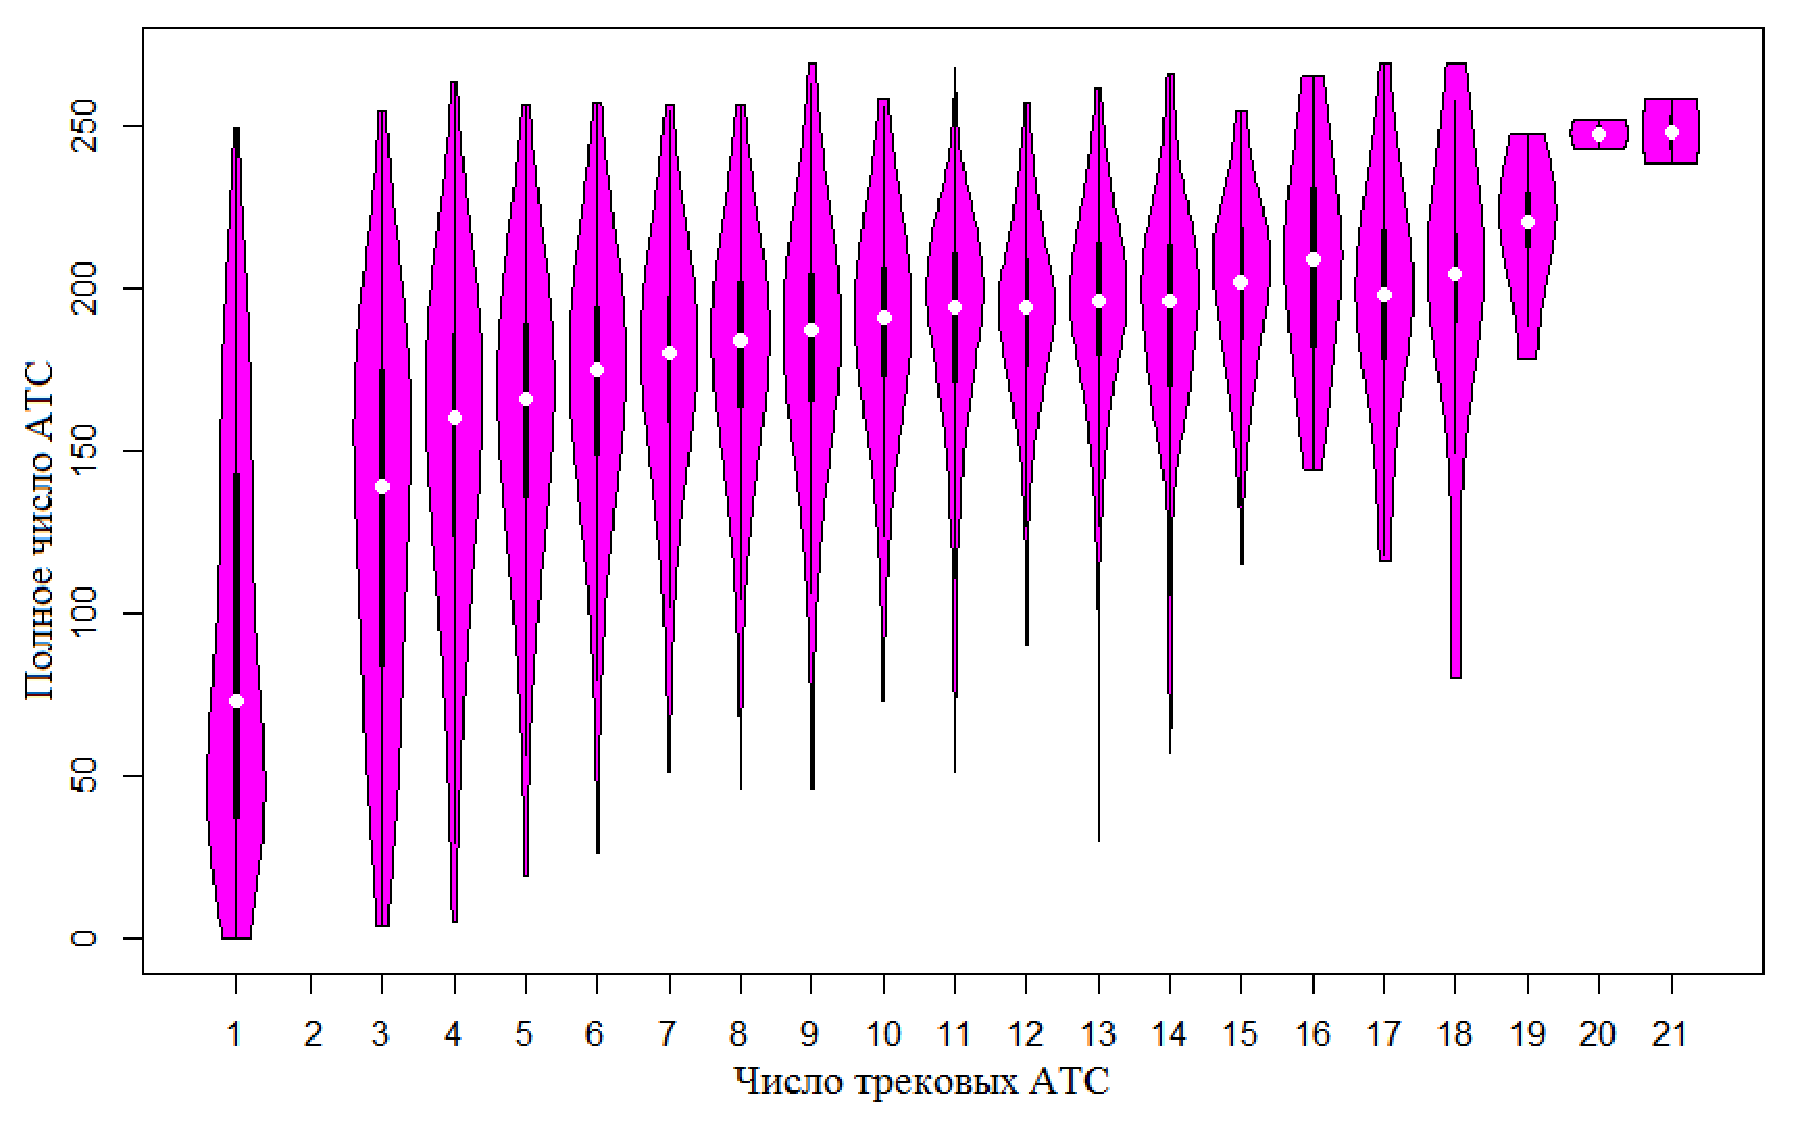
\includegraphics[width=\linewidth]{Vioplot_Detector-Yandex.eps}
\caption{Скрипичная диаграмма зависимости полного числа АТС от числа трековых АТС.}
\label{fig:violin}
\end{center}
\end{figure}

Также, кроме модели вида~\eqref{eq::f_form} были рассмотрены и другие модели, такие как модель числа трековых АТС:
\begin{equation}
    f(\mathbf{a} | N_{\text{track}, i}) = a_0 + a_1N_{\text{track}, i},
    \label{eq::model_N}
\end{equation}
модель числа АТС и скорости
\begin{equation}
    f(\mathbf{a} | N_{\text{track}, i}, V_{\text{est}, i}) = a_0 + a_1N_{\text{track}, i} + a_2V_{\text{est}, i},
    \label{eq::model_NV}
\end{equation}
и модель с логарифмом числа АТС и скоростью
\begin{equation}
    f(\mathbf{a} | N_{\text{track}, i}, V_{\text{est}, i}) = a_0 + a_1\log\left({N_{\text{track}, i}}\right) + a_2V_{\text{est}, i}.
    \label{eq::model_logNV}
\end{equation}


\section{Алгоритм восстановления суммарного потока на въездах и съездах}
Алгоритм восстановления суммарного потока на въездах и съездах состоит из следующих шагов:
\begin{itemize}
  \item Задать перекресток, на котором будет решаться задача восстановления суммарного потока, и определить сегменты, соответствующие въездам и съездам, а также сегменты с которых берутся данные о $N_\text{ain}, N_\text{aout}$.
  \item Определить въезды и съезды принадлежащие множества $K_\text{intrack}, K_\text{outtrack}$.
  Уже имеющееся на них небольшое число данных используем для определения параметров случайного Пуассоновского процесса, соответствующего данному въезду или съезду.
  \item Используя полученные распределения на въездах и съездах из множеств $K_\text{intrack}, K_\text{outtrack}$ вместо реальных данных, а также данные с самого МКАД (которые мы считаем верно восстановленными в разделе~5.2) и данные с въездов и съездов из множеств $K_\text{indet}, K_\text{outdet}$ решаем задачу~\eqref{eq::in_out_quest}.
\end{itemize}
Для решения поставленной задачи предлагается использовать алгоритм~\ref{alg::balance}, использующий понятие дисбаланса $N = N_\text{ain} + N_\text{in} - N_\text{aout} - N_\text{out}$.
Также введём следующие обозначения $max\_cars\_in = k\cdot max\_cars\_per\_enter/exit$~--- максимальное число въезжающих по въездам АТС, $max\_cars\_out = k'\cdot max\_cars\_per\_enter/exit$~--- максимальное число съезжающих по съездам АТС, где $max\_cars\_per\_enter/exit$~--- максимальное число АТС которые могут проехать по съезду/въезду за две минуты, $k$~--- число въездов, $k'$~--- число съездов.
Значение $max\_cars\_per\_enter/exit$ равно 60 АТС~\cite{introductionMathMod}, то есть 1 АТС за каждые две секунды.
\begin{algorithm}[!ht]
 \caption{Алгоритм восстановления суммарных значений потока на въездах/съездах использующий уравнение баланса}
 \label{alg::balance}
 \begin{algorithmic}
 \IF {$N \neq 0$}
  \IF{$N > 0$}
   \STATE $max\_extra\_cars = N_\text{out} + (max\_cars\_in - N_\text{in})$
   \IF{$N < max\_extra\_cars$}
    \STATE $N_\text{estout} = N_\text{out} - N \cdot N_\text{out} / max\_extra\_cars$
    \STATE $N_\text{estin} = N_\text{in} + N \cdot (max\_cars\_in - N_\text{in}) / max\_extra\_cars$
   \ELSE
    \STATE $N_\text{estout} = 0$
    \STATE $N_\text{estin} = max\_cars\_in$
   \ENDIF
  \ELSE
   \STATE $max\_extra\_cars = N_\text{in} + (max\_cars\_out - N_\text{out})$
   \IF{$|N| < max\_extra\_cars$}
    \STATE $N_\text{estin} = N_\text{in} - N \cdot N_\text{in} / max\_extra\_cars$
    \STATE $N_\text{estout} = N_\text{out} + N \cdot (max\_cars\_out - N_\text{out}) / max\_extra\_cars$
   \ELSE
    \STATE $N_\text{estin} = 0$
    \STATE $N_\text{estout} = max\_cars\_out$
   \ENDIF
  \ENDIF
 \ENDIF
 \end{algorithmic}
\end{algorithm}

\section{Вычислительный эксперимент}
\label{sec::experiments}
В работе проведён вычислительный эксперимент на реальных данных с МКАДа за 2012 год и проверен предложенный подход к агрегации данных с автомагистралей.

\subsection{Описание данных}
В данной работе используются данные с GPS-треков и дорожных датчиков за 2012 год
Данные с GPS-треков представляют собой набор сегментов, каждый из которых соотносится с некоторым участком автодороги.
Объединение сегментов покрывает весь рассматриваемый участок транспортной сети.
Для каждого сегмента известно число проехавших за двухминутный интервал трековых АТС $N_\text{track}$ и среднее время их проезда по нему, из которого впоследствии рассчитывается скорость $V_\text{track}$.
Также если за две минуты по данному сегменту проехало менее трех трековых АТС, то они не учитываются.

Для каждого датчика известно его местоположение на автомагистрали.
Данные с датчиков состоят из числа проехавших за две минуты АТС $N_\text{det}$ для каждой из полос и их скорости $V_\text{det}$.
Заметим, что в данных с датчиков также могут быть ошибки, например на рис.~\ref{fig:baddet} показаны данные датчика, в которых отсутствуют записи за 4 часа.
\begin{figure}[!ht]
\begin{center}
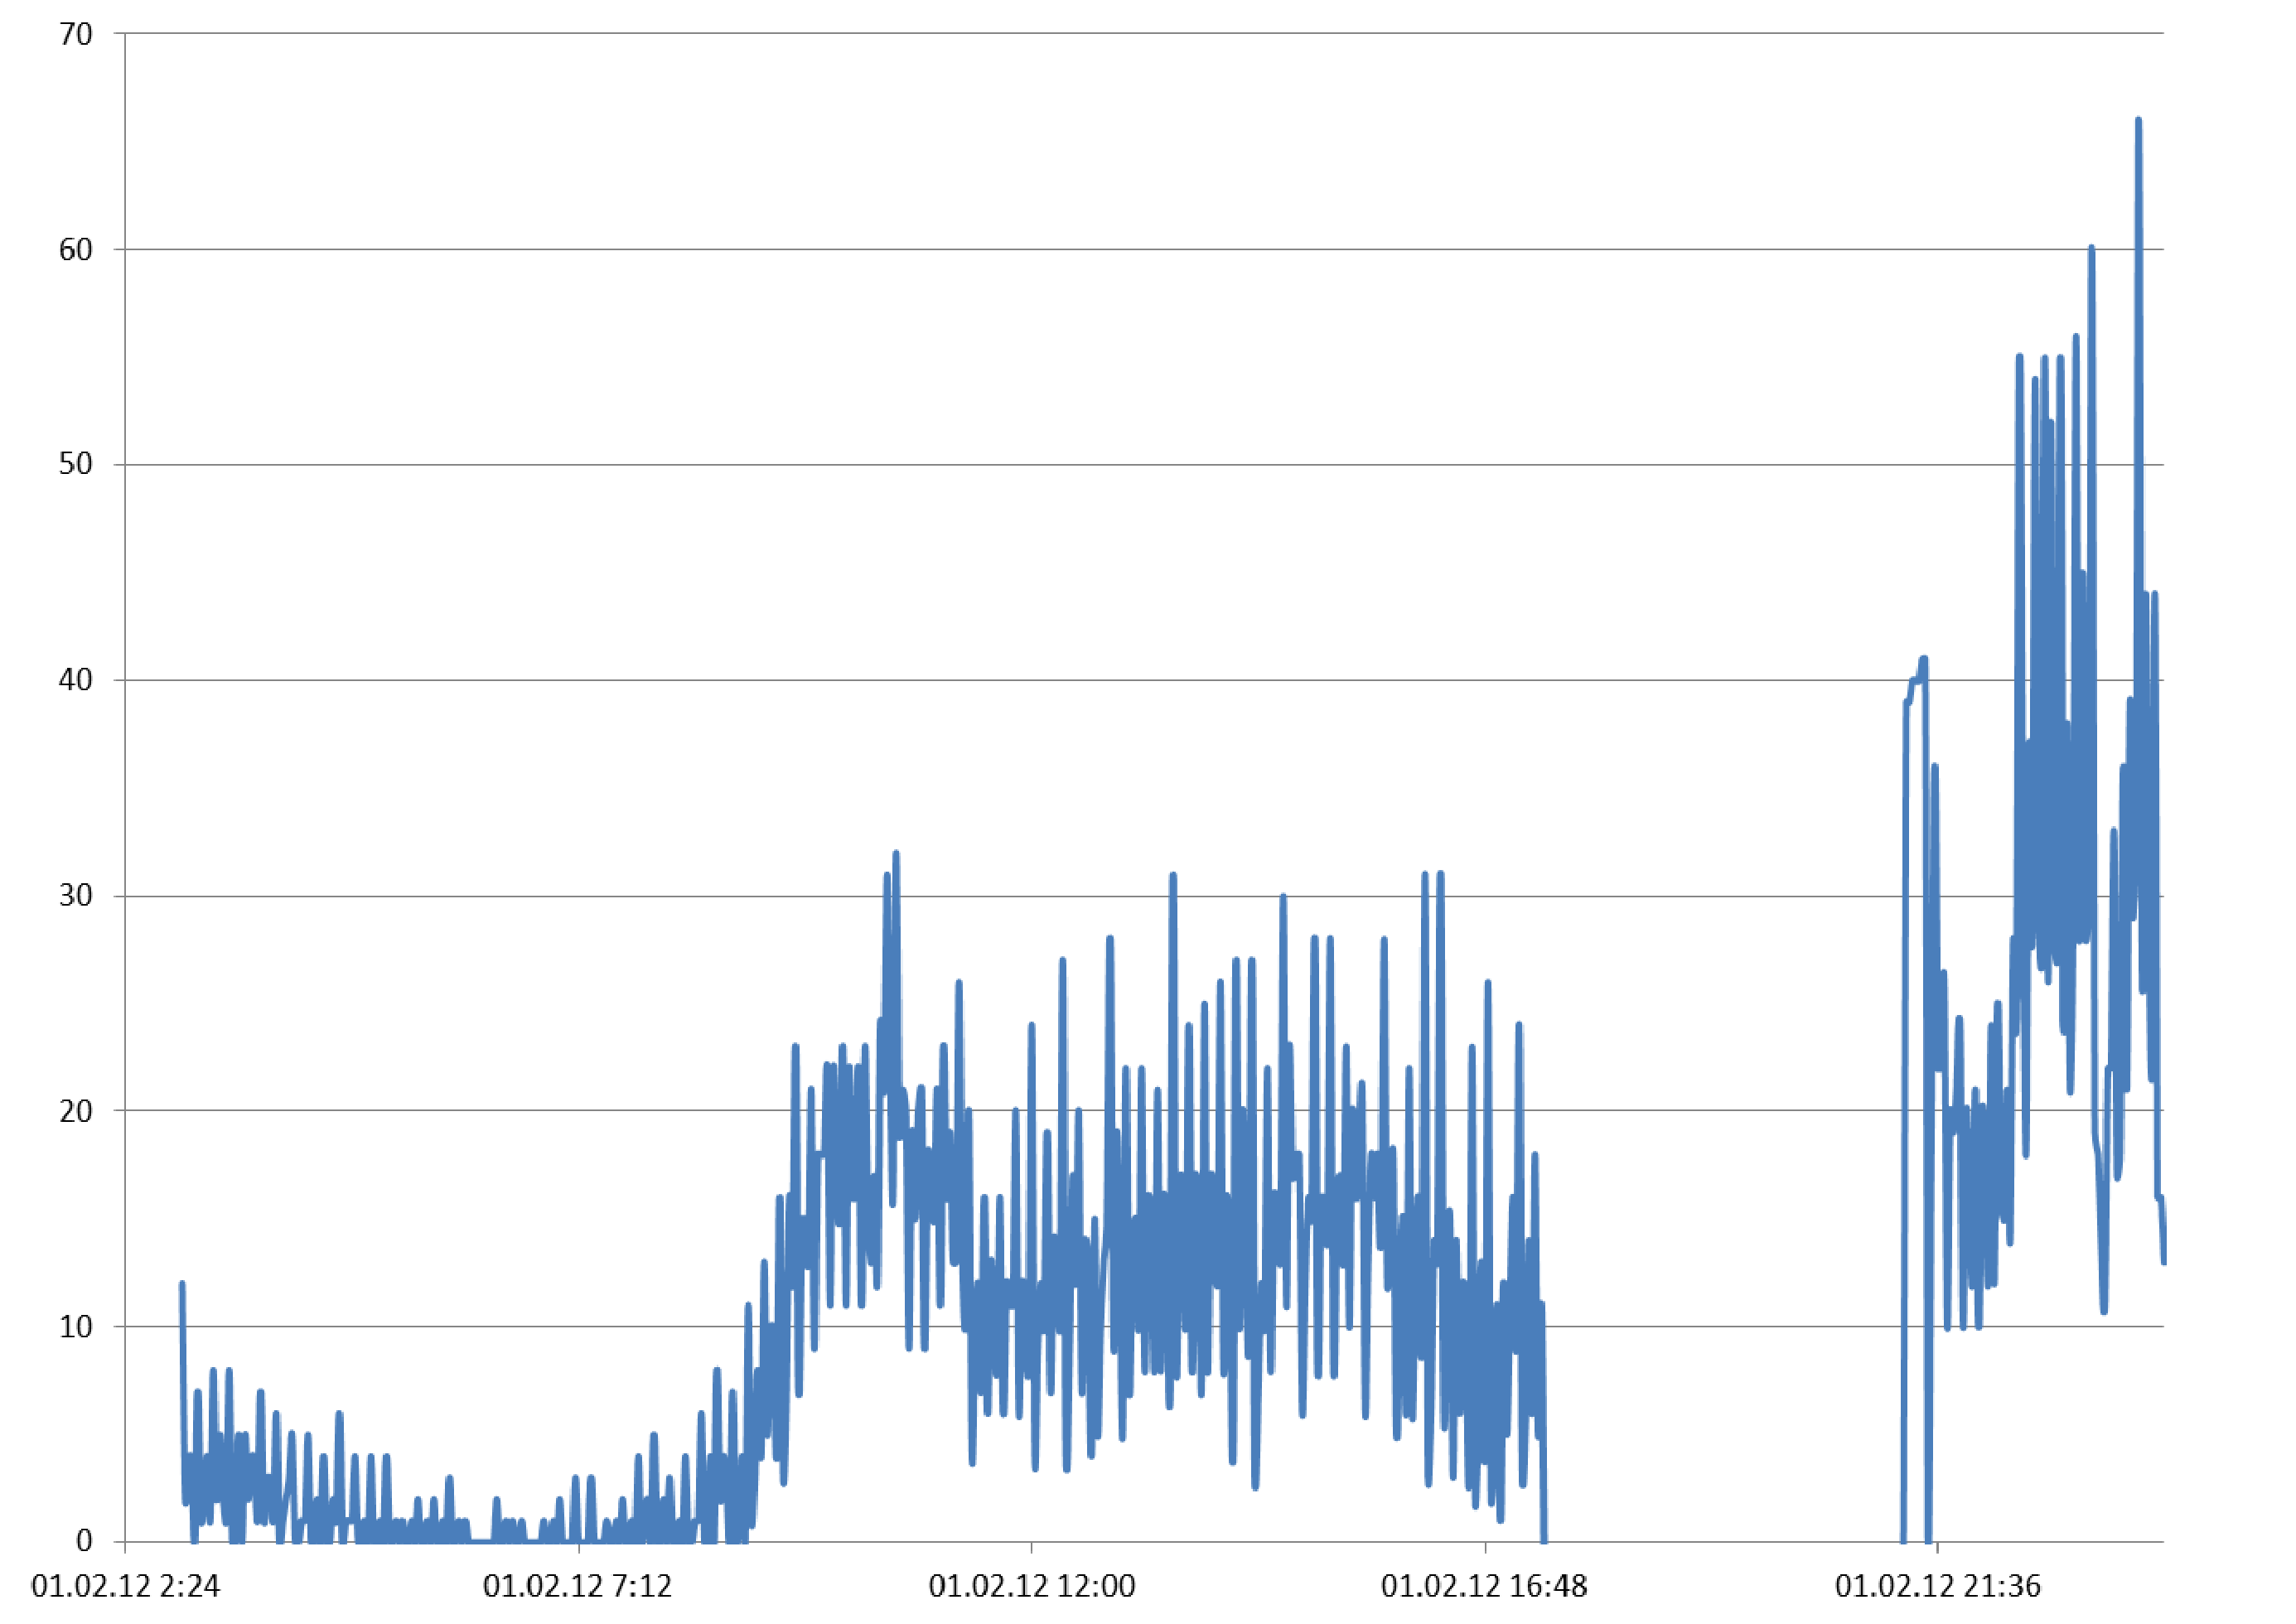
\includegraphics[width=1\linewidth]{Bad_detector_example.eps}
\caption{Число зарегистрированных датчиком АТС в зависимости от времени суток. Детектор перестаёт фиксировать АТС в 17:25 и начинает в 21:15.}
\label{fig:baddet}
\end{center}
\end{figure}


\subsection{Эксперимент на автомагистрали}
В экспериментах вместо числа АТС использовалась плотность АТС, чтобы учесть различные длины сегментов.
Обозначим плотность АТС на участке автомагистрали, полученную с помощью данных дорожных датчиков $\rho_{det} = N_\text{det} / l$, где $l$~--- длина участка автомагистрали в данных GPS-треков.
% \rho_{est} = N_\text{est} / l
$\boldsymbol{\rho}_\text{est} \in \mathbb{R}_{+}^{n}, \boldsymbol{\rho}_\text{det} \in \mathbb{R}_{+}^{n}$~--- вектора соответсвующих по времени значений $\rho_\text{est}, \rho_\text{det}$, где $n$~--- число двухминутных интервалов в выбранном временном промежутке.

Для решения задачи~\eqref{eq::complex_error_func} необходимо сначала получить преобразование скорости, решив задачу~\eqref{eq::speed_error_function}.
Решением задачи~\eqref{eq::speed_error_function} явлется следующее выражение:
\begin{equation}
    V_\text{est} = 12.34 + 0.639V_\text{track}.
    \label{eq::speed_transform}
\end{equation}

На рис.~\ref{fig:with_without_V} показана зависимость плотности АТС от времени суток в случае использования преобразования~\eqref{eq::speed_transform} (слева) и в случае использования скоростей, полученных с GPS-треков $V_\text{track}$ (справа).
При использовании преобразования~\eqref{eq::speed_transform} ошибка аппркосимации на обучении $\sigma(\mathbf{a_1}|\mathbf{\rho}_\text{track}, \mathbf{V}_\text{est}, \mathbf{\rho}_\text{det}) = 0.03$ и корреляция $corr(\mathbf{\rho}_\text{est}, \mathbf{\rho}_\text{det}) = 0.787$, в то время как при использовании данных с GPS-треков ошибка аппроксимации $\sigma(\mathbf{a_2}|\mathbf{\rho}_\text{track}, \mathbf{V}_\text{track}, \mathbf{\rho}_\text{det}) = 0.042$ и корреляция $corr(\mathbf{\rho}_\text{est}, \mathbf{\rho}_\text{det}) = 0.672$.
Это означает, что использование преобразования~\eqref{eq::speed_transform} повышает качество аппроксимации.

\begin{figure}[!ht]
\subfloat{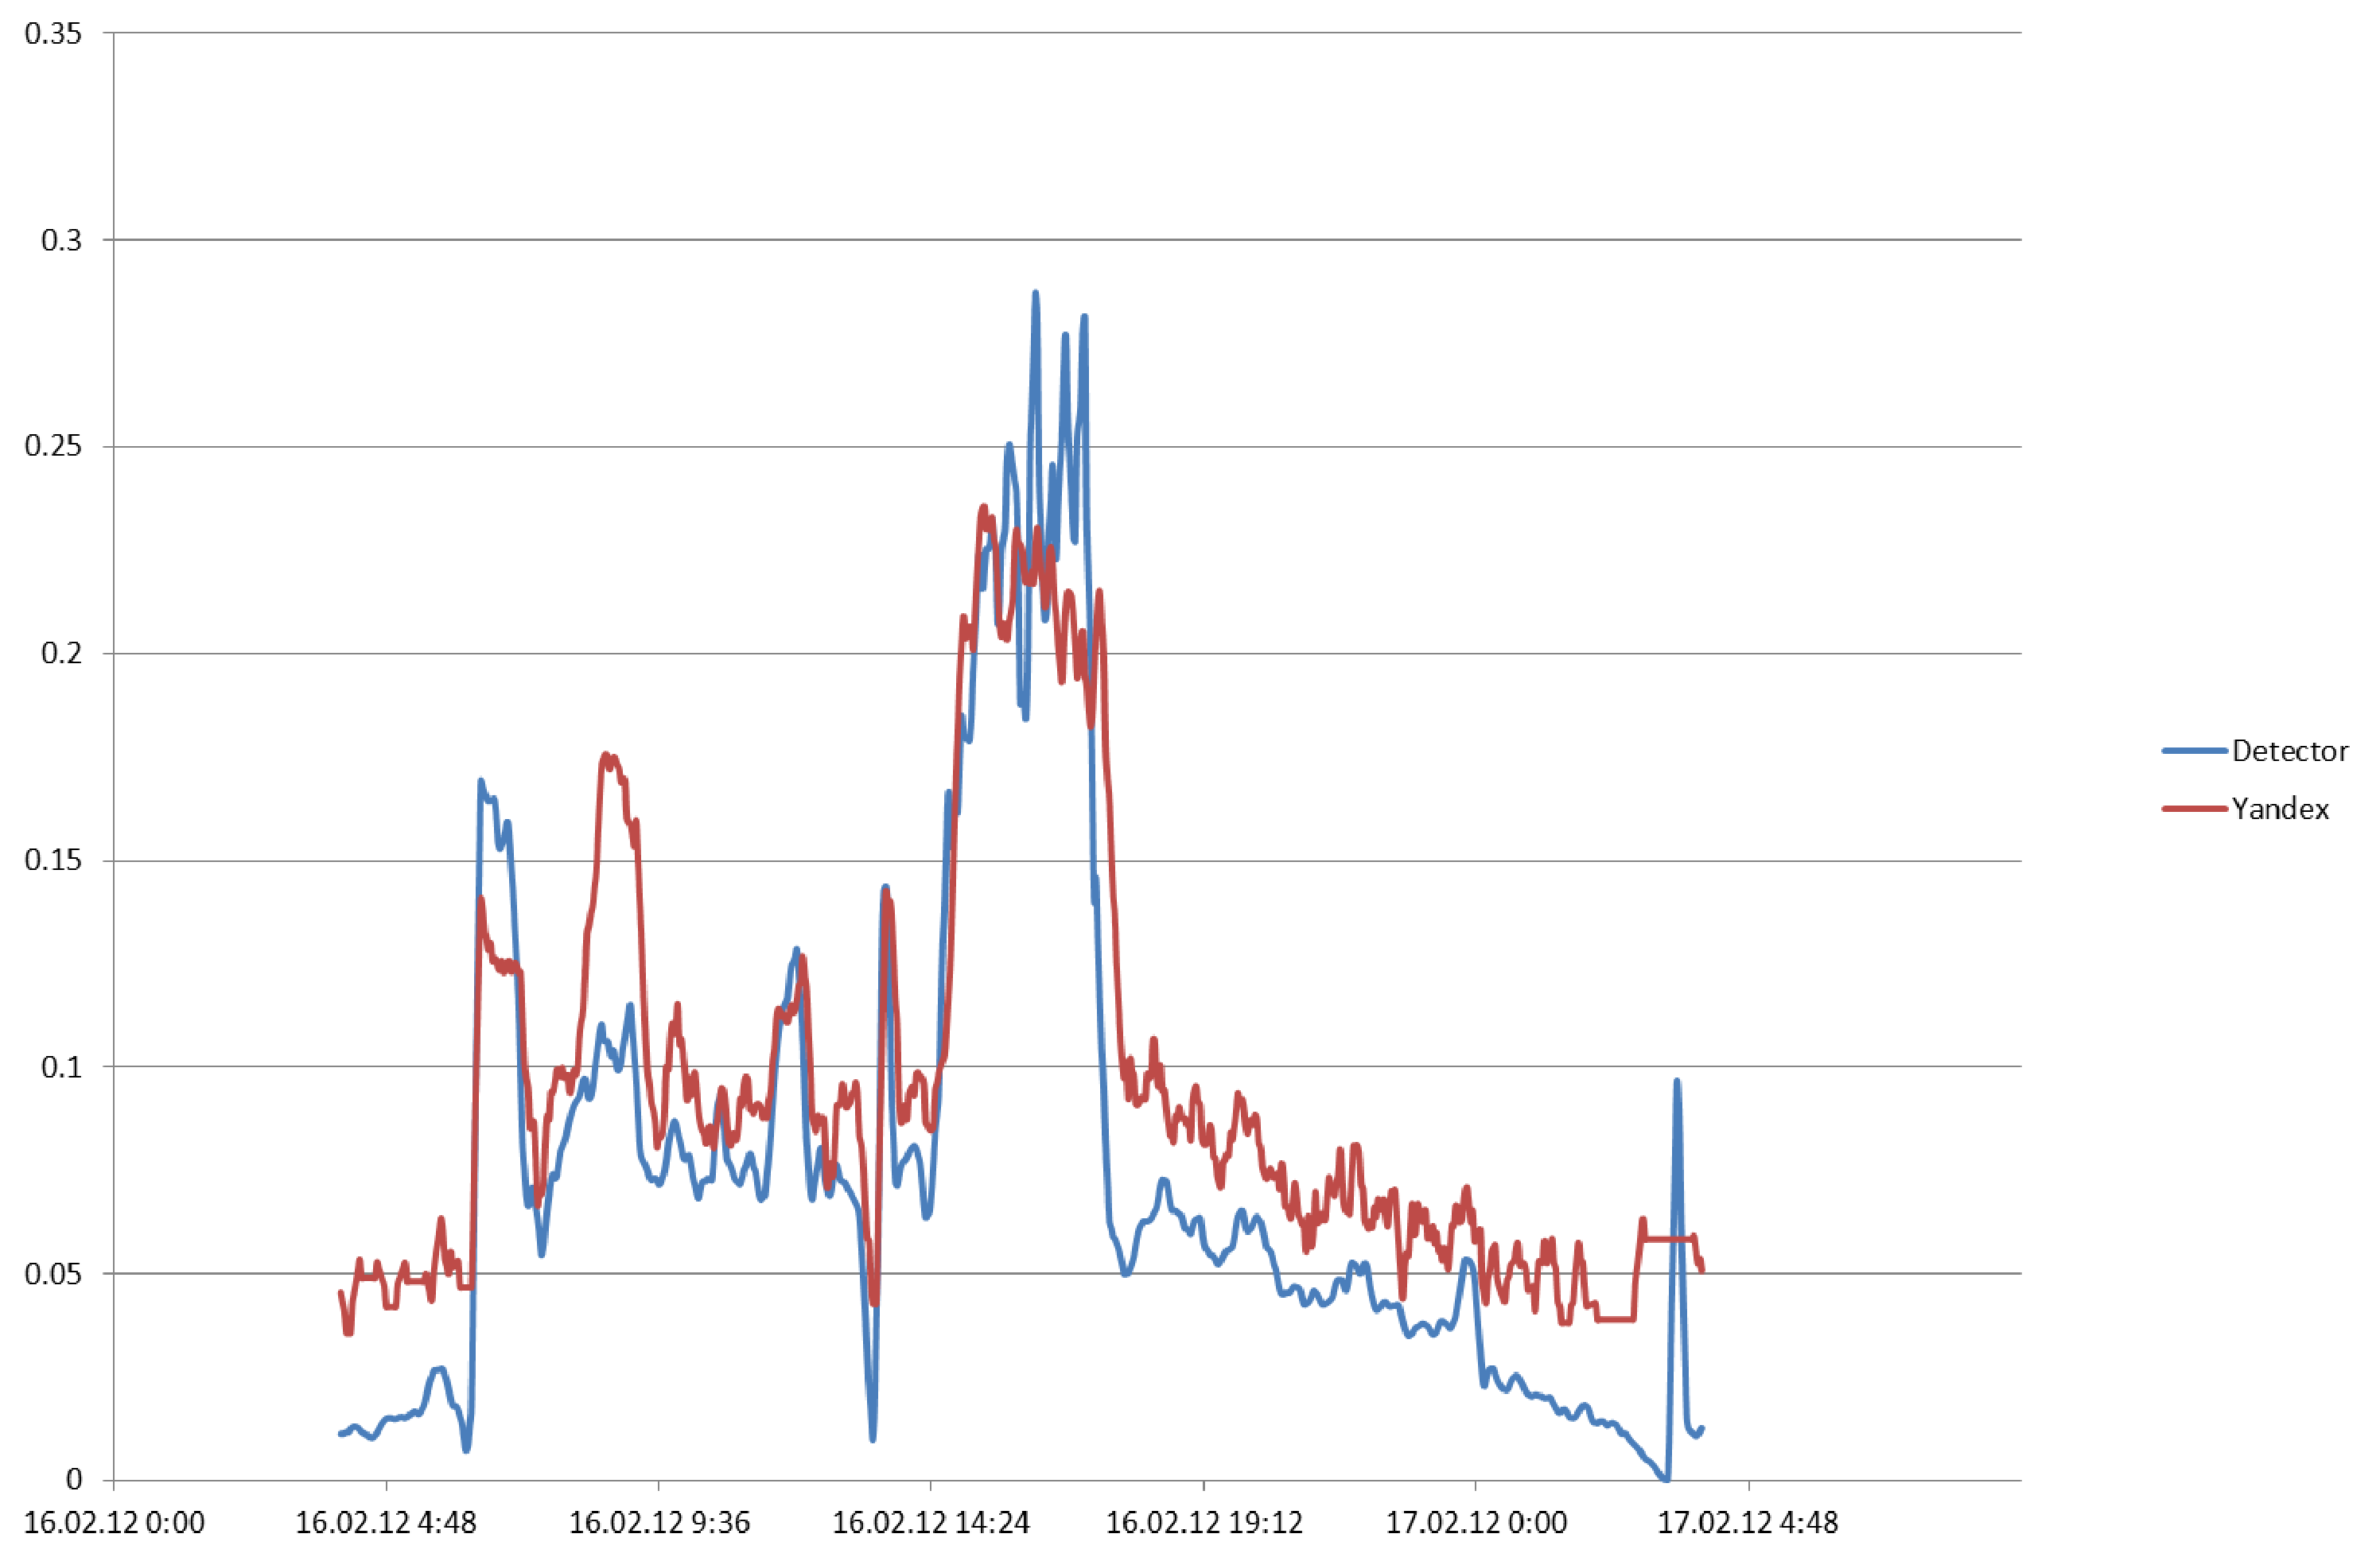
\includegraphics[width=0.5\linewidth]{With_V.eps}}
\subfloat{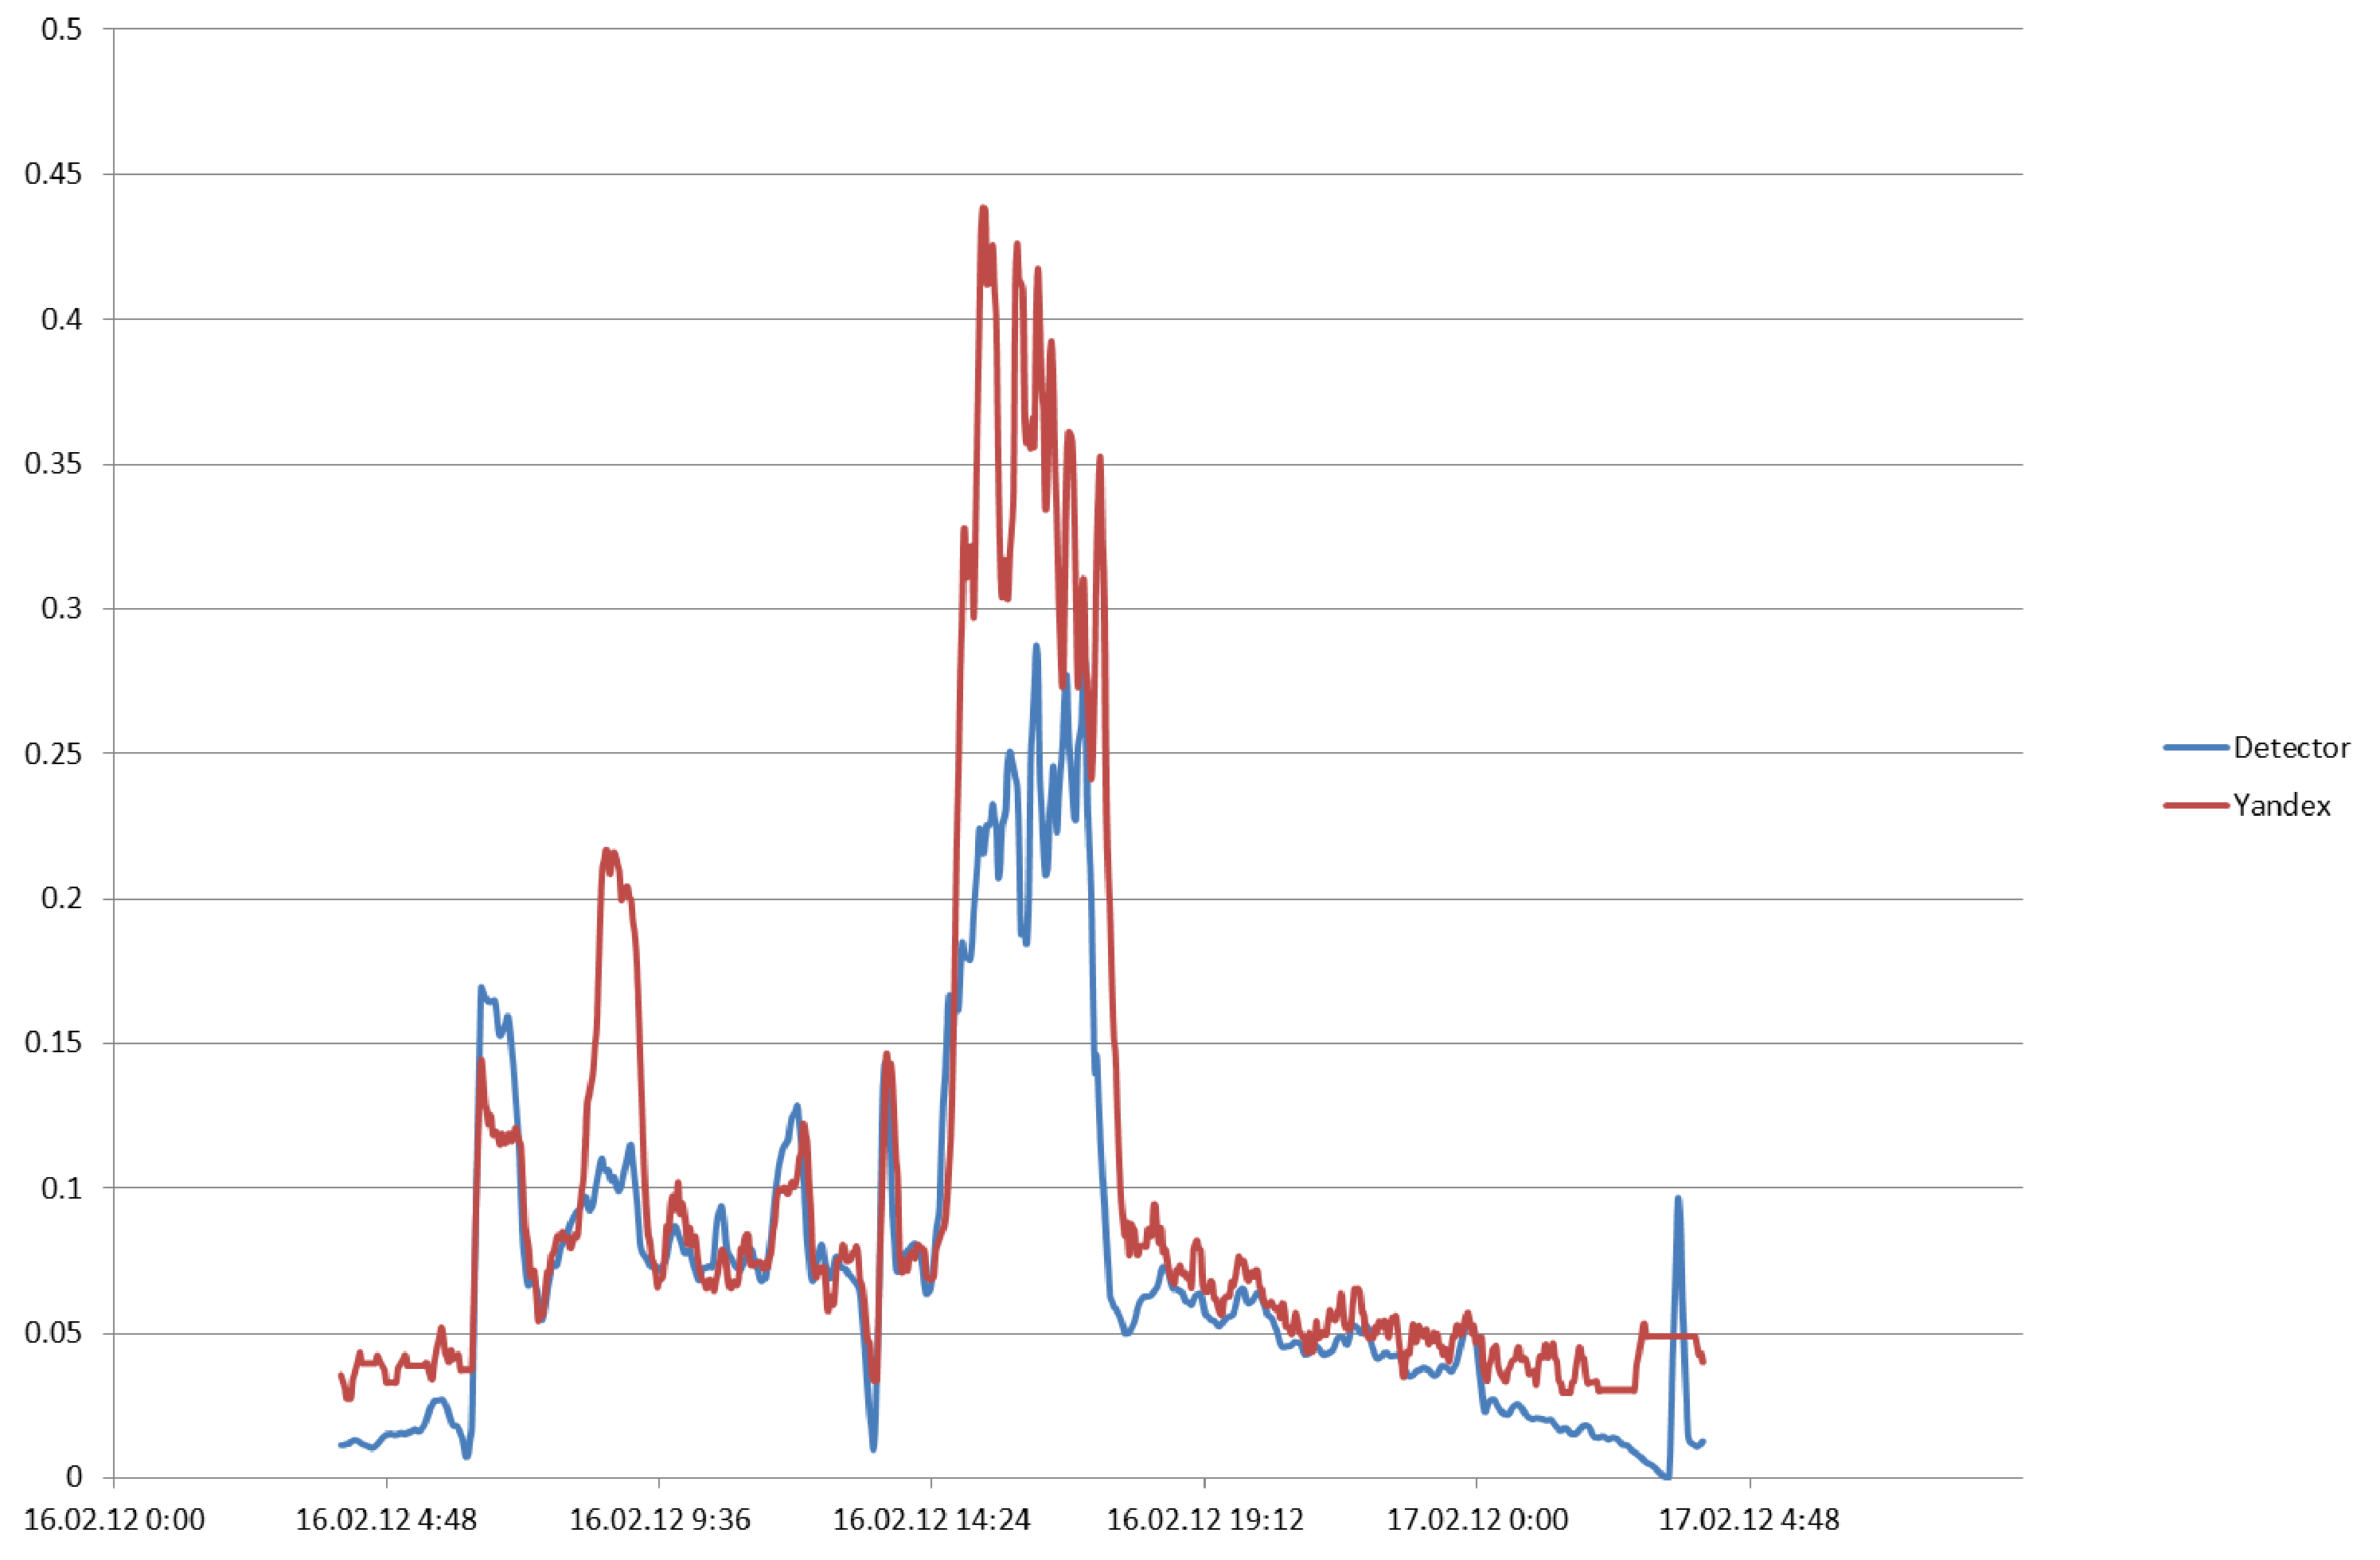
\includegraphics[width=0.5\linewidth]{Without_V.eps}}
\caption{Графики полученных с помощью моделей плотностей в случае с использованием модели для скорости (слева) и без (справа).}
\label{fig:with_without_V}
\end{figure}

Далее рассмотрим метод улучшения качества аппроксимации с помощью построения нескольких моделей для данных с различными значениями плотности АТС, определяемыми по данным датчиков.
Для этого возьмём множество данных за февраль $L$ для датчика и подсегмента под ним и выделим из них множество $H \subset L$~---данные, соответствующие плотности АТС более 0.05 АТС/м, которая является переходной между фазами свободного и синхронизированного потока для МКАД~\cite{collectiveArticle}.

Задача~\eqref{eq::complex_error_func} решается для данных $L$ и $H$ отдельно с получением векторов параметров $\mathbf{a}_L, \mathbf{a}_H$ соответственно.
Решением задачи~\eqref{eq::complex_error_func} на данных $H$ является следующее выражение:
\begin{equation}
    N_\text{est} = 157.78 + 4.54N_\text{track} - 4.59\log(N_\text{track}) + 0.153V_\text{est} - 85.069N_\text{track}/V_\text{track},
    \label{eq::model_high}
\end{equation}
а на данных $L$:
\begin{equation}
    N_\text{est} = 117.75 + 2.11N_\text{track} + 41.55\log(N_\text{track}) - 0.327V_\text{est} - 128.89N_\text{track}/V_\text{est}
    \label{eq::model_all}
\end{equation}

Первая модель использовалась при плотности выше 0.1 АТС/м (плотность, соответсвующая началу синхронизированной фазы~\cite{collectiveArticle}), вторая~--- при плотности ниже 0.1 АТС/м.
Корреляция на обучении составила 0.787, средняя ошибка 0.03 и сравнение результата $\rho_\text{det}$ с $\rho_\text{est}$ показано на рис.~\ref{fig:cstudy}.
Для контроля выбраны четыре пары датчик-сегмент и проведены вычисления с использованием моделей~\eqref{eq::model_high}, \eqref{eq::model_all}.
На контроле корреляция составила 0.823, 0.80, 0.85, 0.65, средняя ошибка 0.0363, 0.0382, 0.0339, 0.0393 соответственно и сравнение результата $\rho_\text{det}$ с $\rho_\text{est}$ показано на рис.~\ref{fig:ctest} для одной из тестовых пар.
\begin{figure}[!ht]
\begin{center}
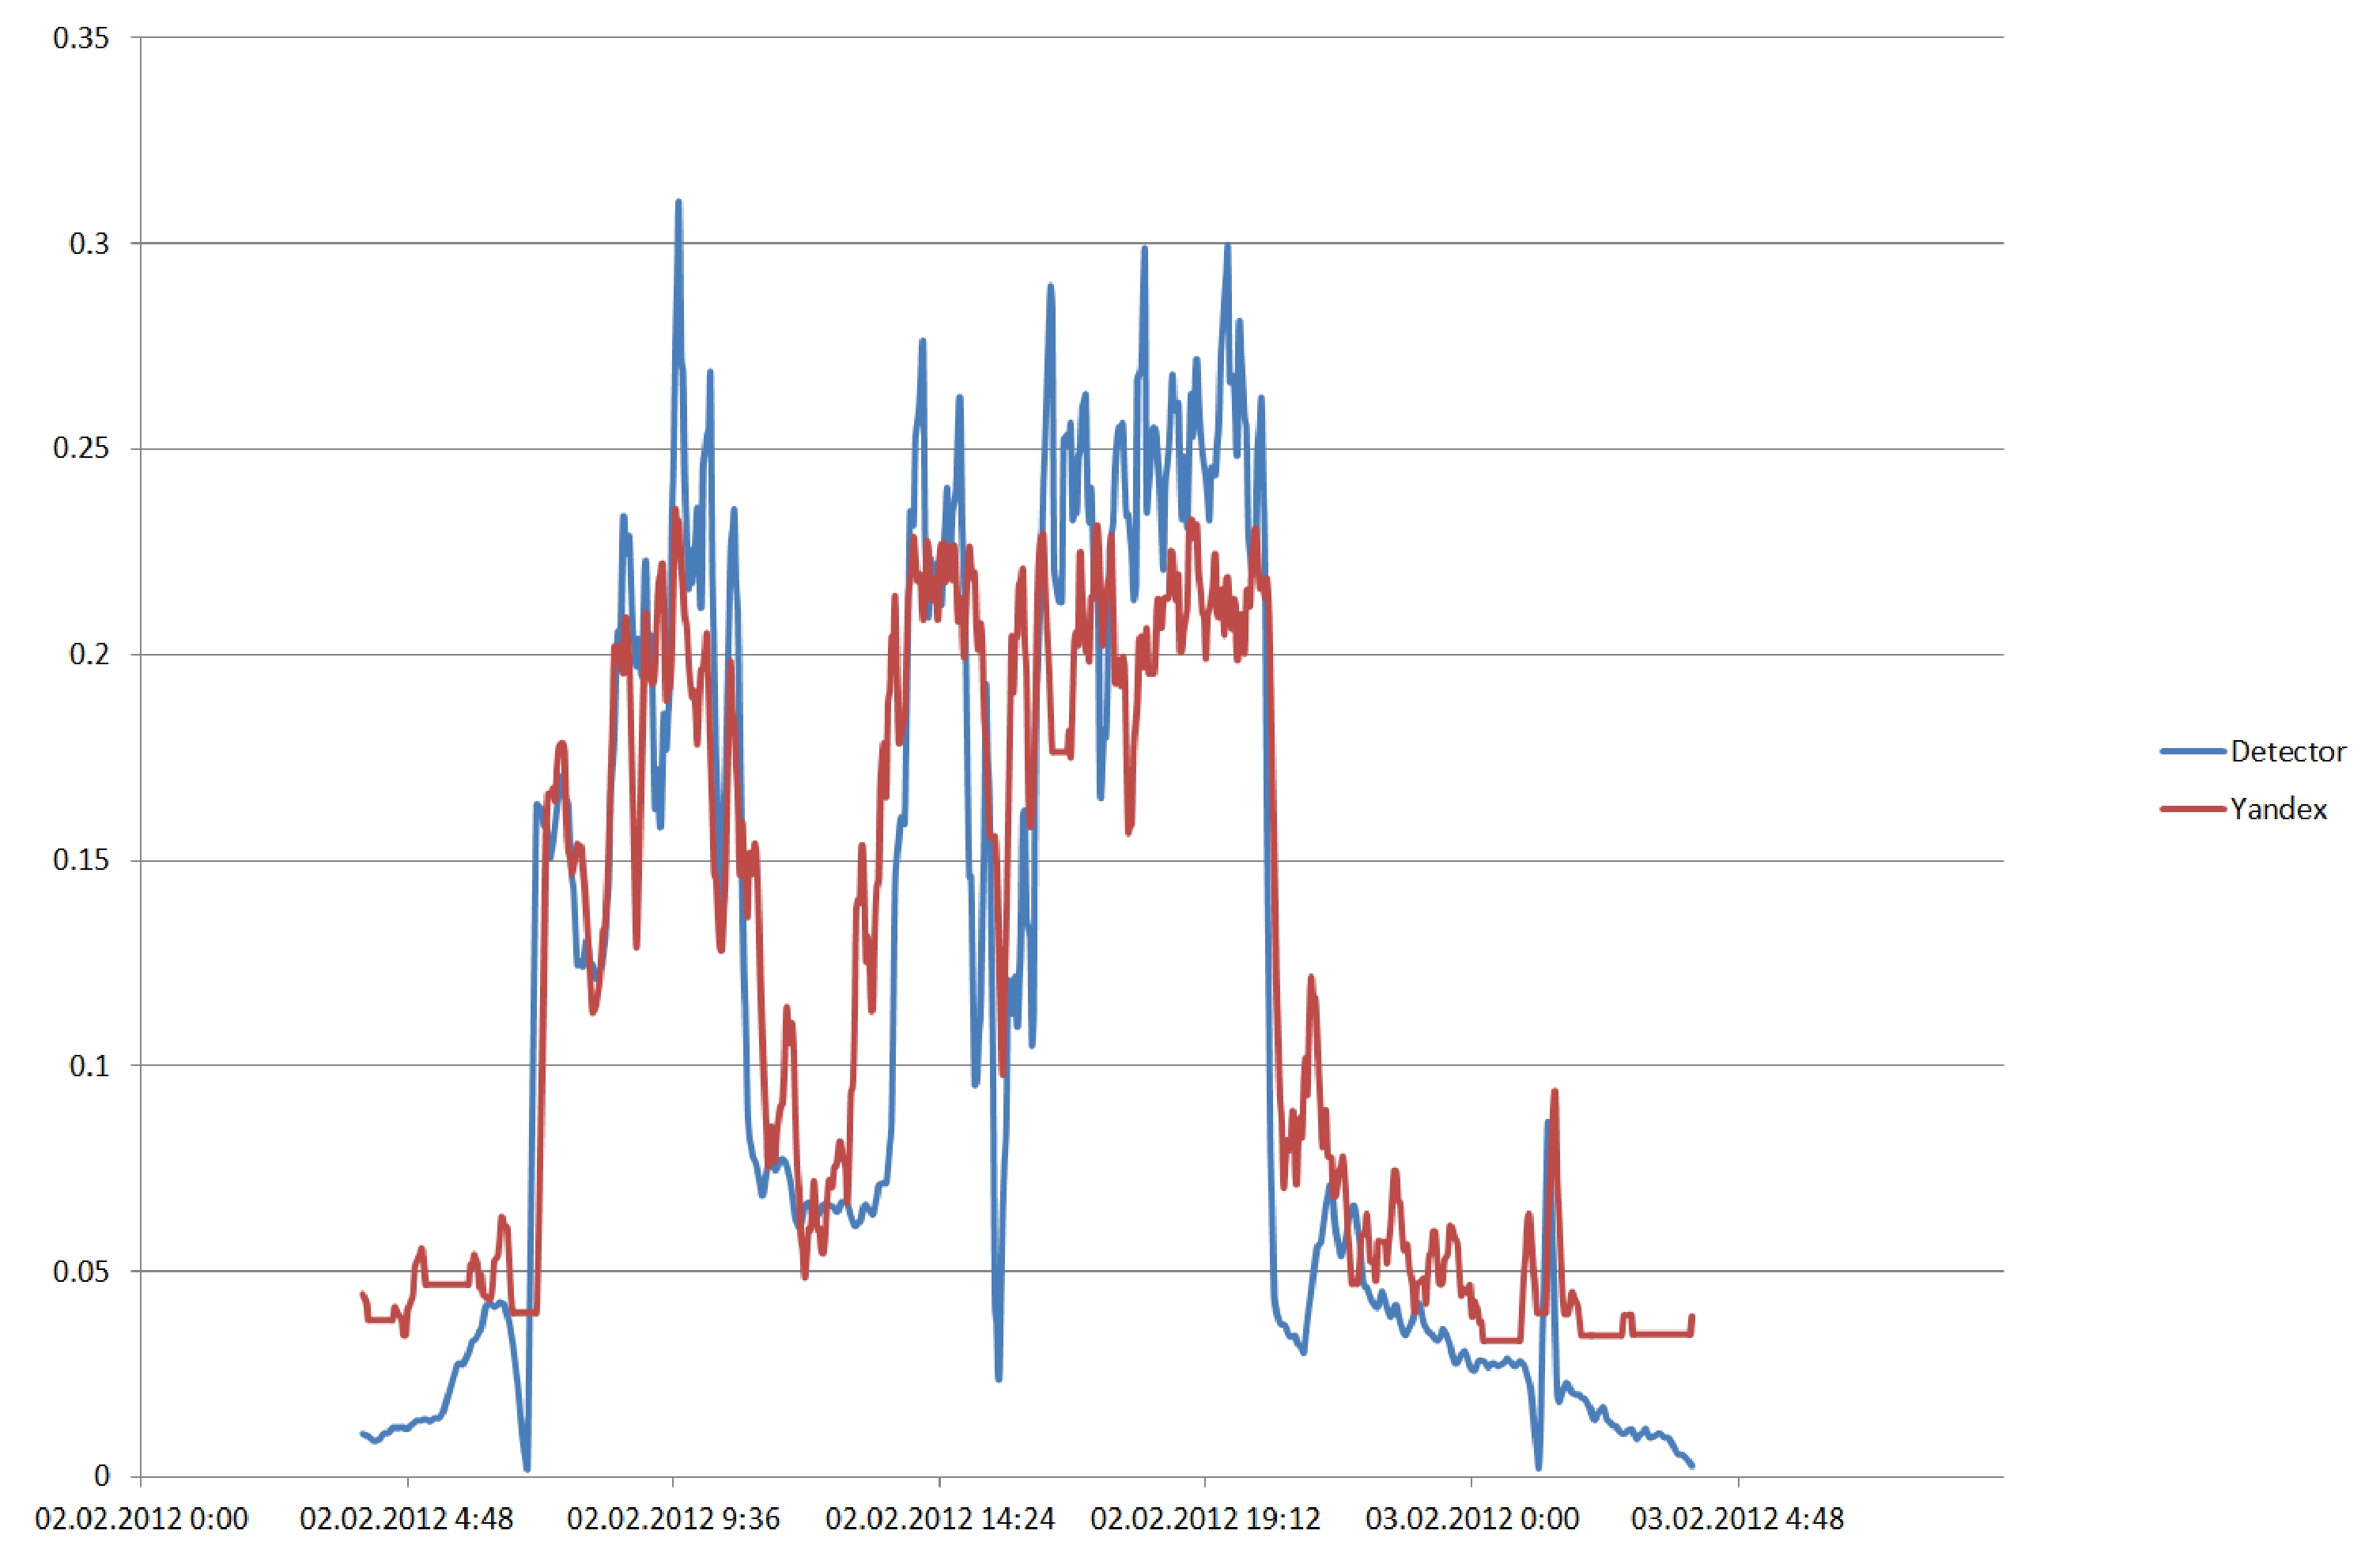
\includegraphics[width=\linewidth]{Complex_Data_Study.eps}
\caption{Средняя за 10 минут плотность АТС рассчитанная по данным датчика и аппроксимированным трековым данным на обучении.}
\label{fig:cstudy}
\end{center}
\end{figure}
\begin{figure}[!ht]
\begin{center}
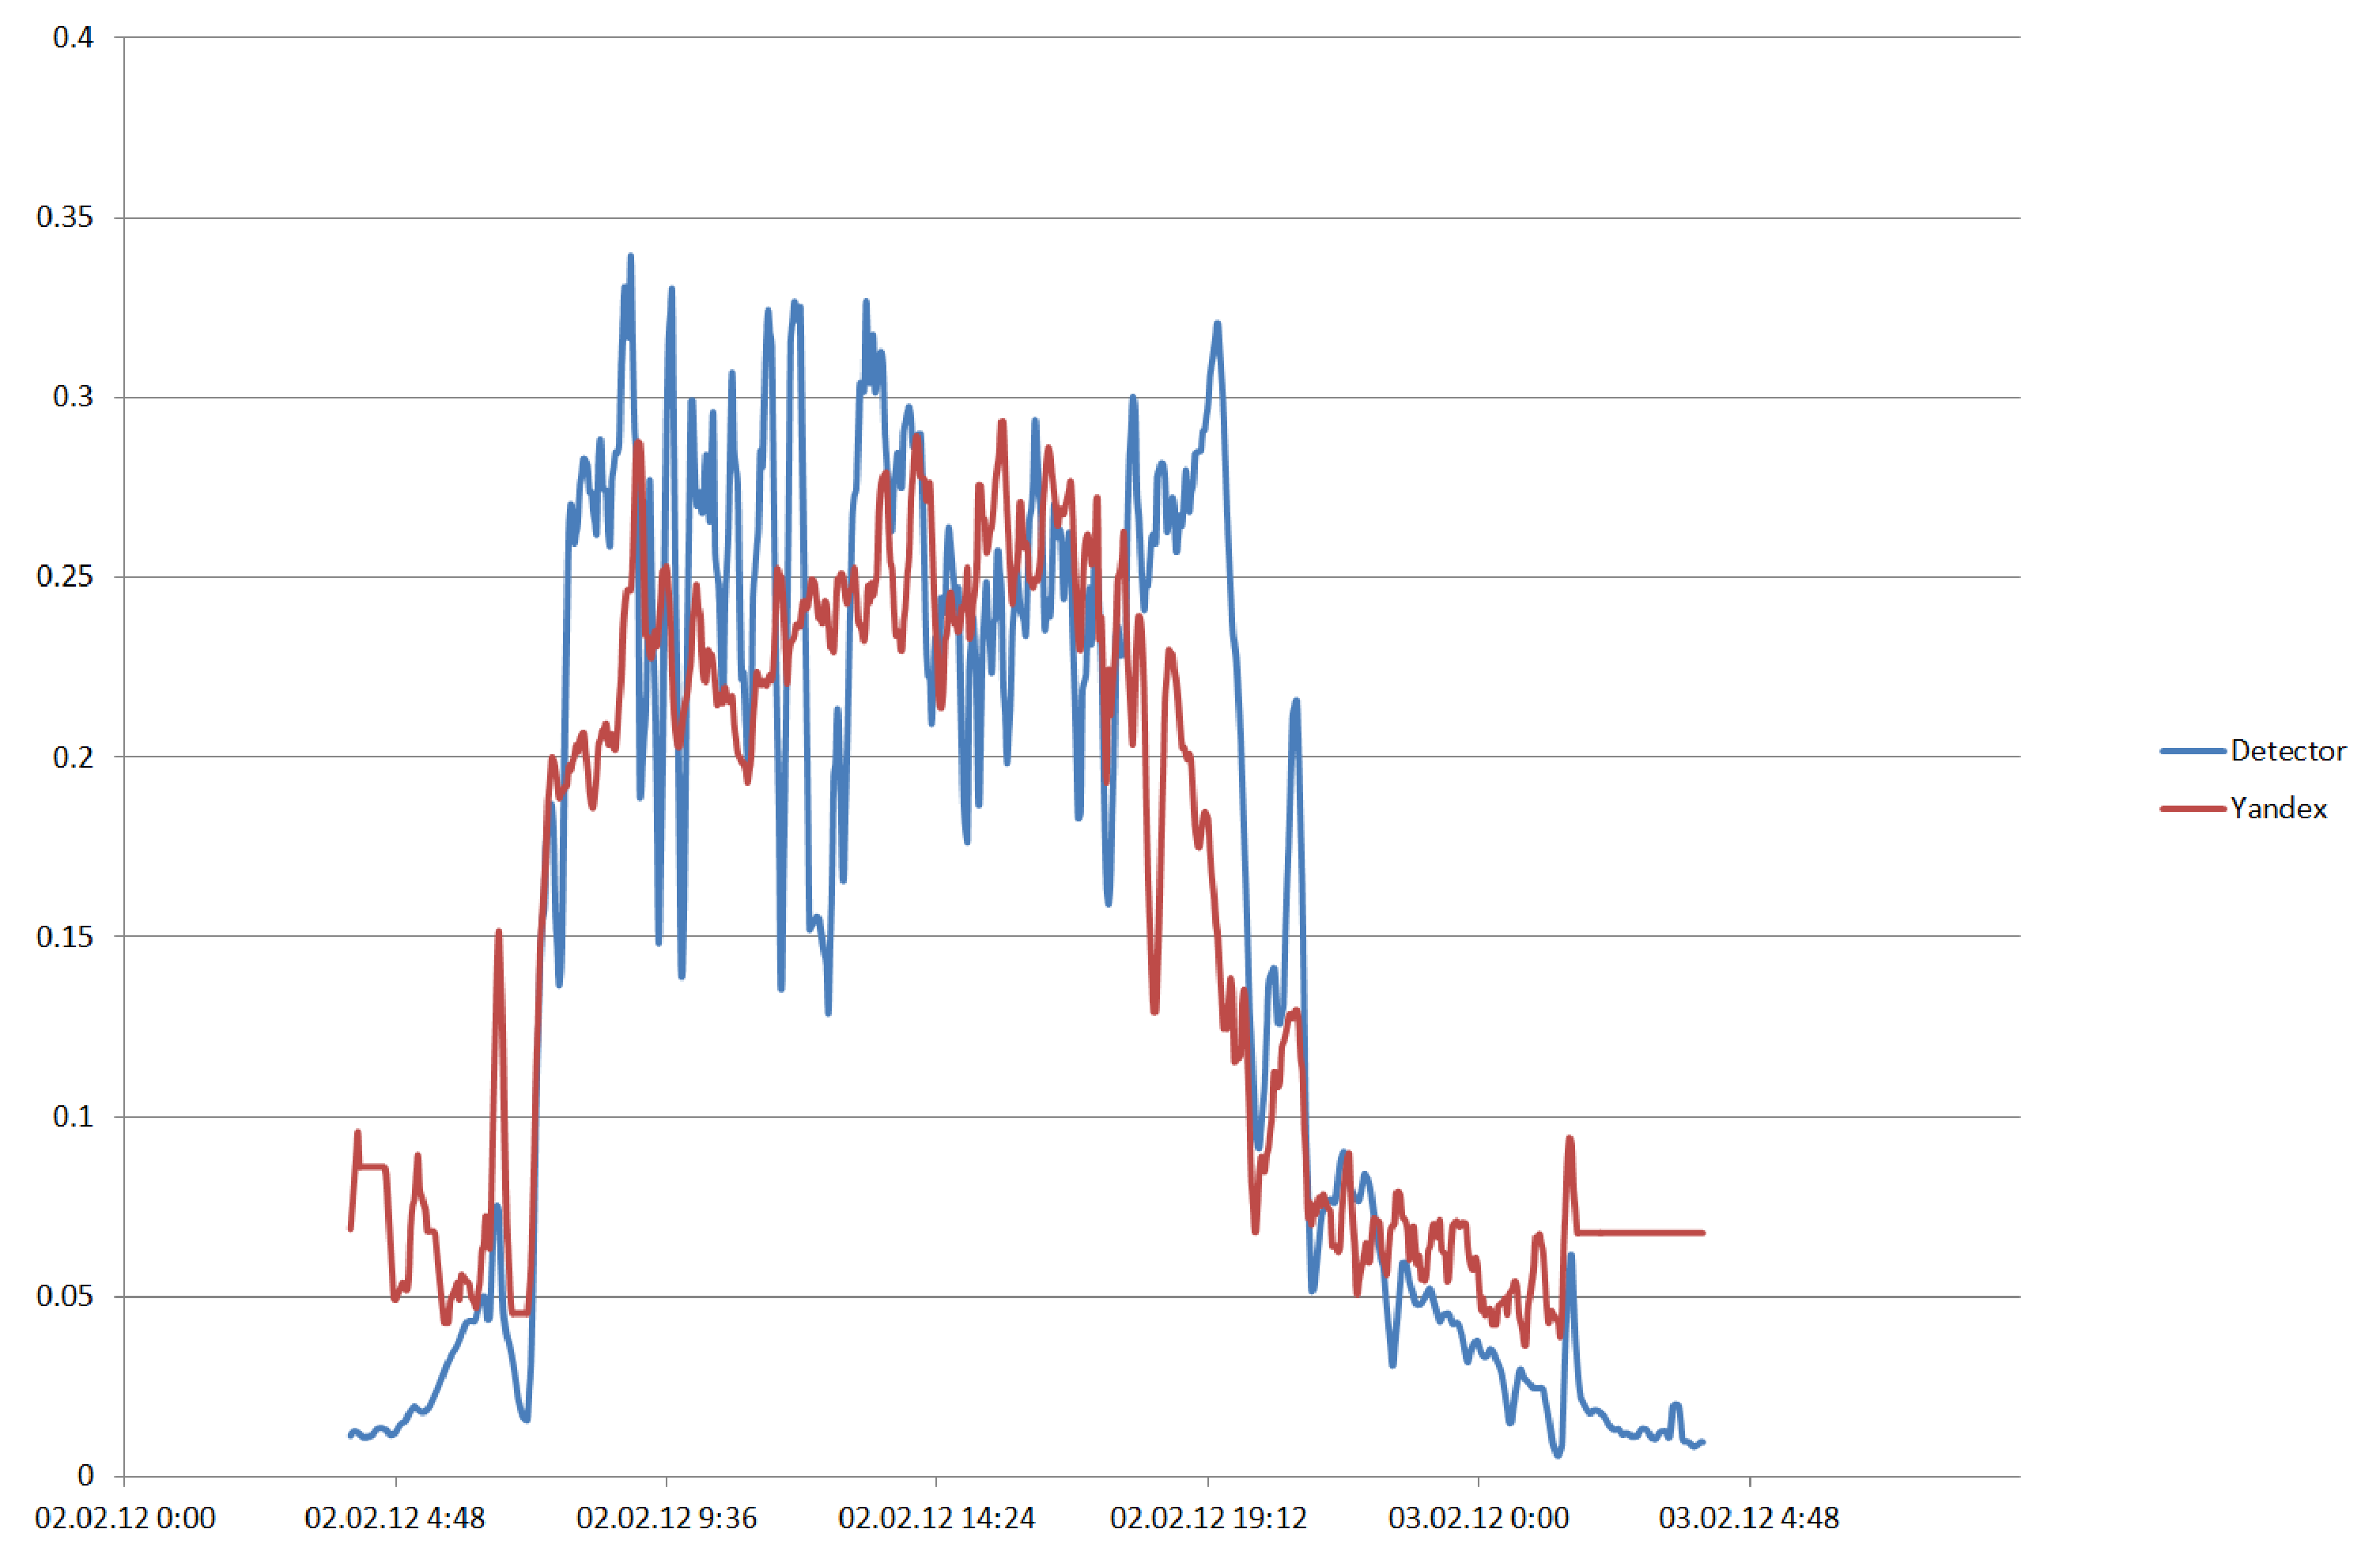
\includegraphics[width=\linewidth]{Complex_Data_Test.eps}
\caption{Средняя за 10 минут плотность АТС рассчитанная по данным датчика и аппроксимированным трековым данным на контроле.}
\label{fig:ctest}
\end{center}
\end{figure}

Также был проведён эксперимент для проверки возможности использования построенной модели для получения оценки количества проехавших АТС в режиме реального времени с использование данных GPS-треков.
Чтобы обучить модель в этом случае, необходимо использовать исторические данные за некоторый промежуток времени до дня, для которого надо получить оценку.
В нашем случае для обучения брались данные за каждые 7 дней перед рассматриваемым днём, который является контрольным временным интервалом.
На рис.~\ref{fig:weeklearn} показана заисимость функции ошибки и коэффициента корреляции от дня на усреднённых за 10 минут данных для построенных моделях для каждого дня.
\begin{figure}[!ht]
\subfloat{\includegraphics[width=0.5\linewidth]{One_week_learn_rho.eps}}
\subfloat{\includegraphics[width=0.5\linewidth]{One_week_learn_err.eps}}
\caption{Корреляция для усреднённых за 10 минут данных и среднеквадратичная ошибка на контроле для эксперимента с обучением по 7 дням.}
\label{fig:weeklearn}
\end{figure}


На рис.~\ref{fig:cN},~\ref{fig:cNV},~\ref{fig:clogNV} показаны результаты работы моделей~\eqref{eq::model_N},~\eqref{eq::model_NV},~\eqref{eq::model_logNV}.
Сравнение рассматриваемых моделей приведено в таблице~\ref{tab::model_compare}. Из таблицы~\ref{tab::model_compare} следует, что лучшей является модель~\eqref{eq::f_form}.

В таблице~\ref{tab::model_compare_high} приведено сравнение среднеквадратической ошибки моделей~\eqref{eq::f_form},\eqref{eq::model_N},~\eqref{eq::model_NV},~\eqref{eq::model_logNV} при большой плотности $\rho_\text{det}>0.2$. Из таблицы~\ref{tab::model_compare_high} следует, что модель~\eqref{eq::f_form} значительно лучше при больших плотностях, чем модели~\eqref{eq::model_N},~\eqref{eq::model_logNV} и лучше модели~\eqref{eq::model_NV}.


\begin{figure}[!ht]
\begin{center}
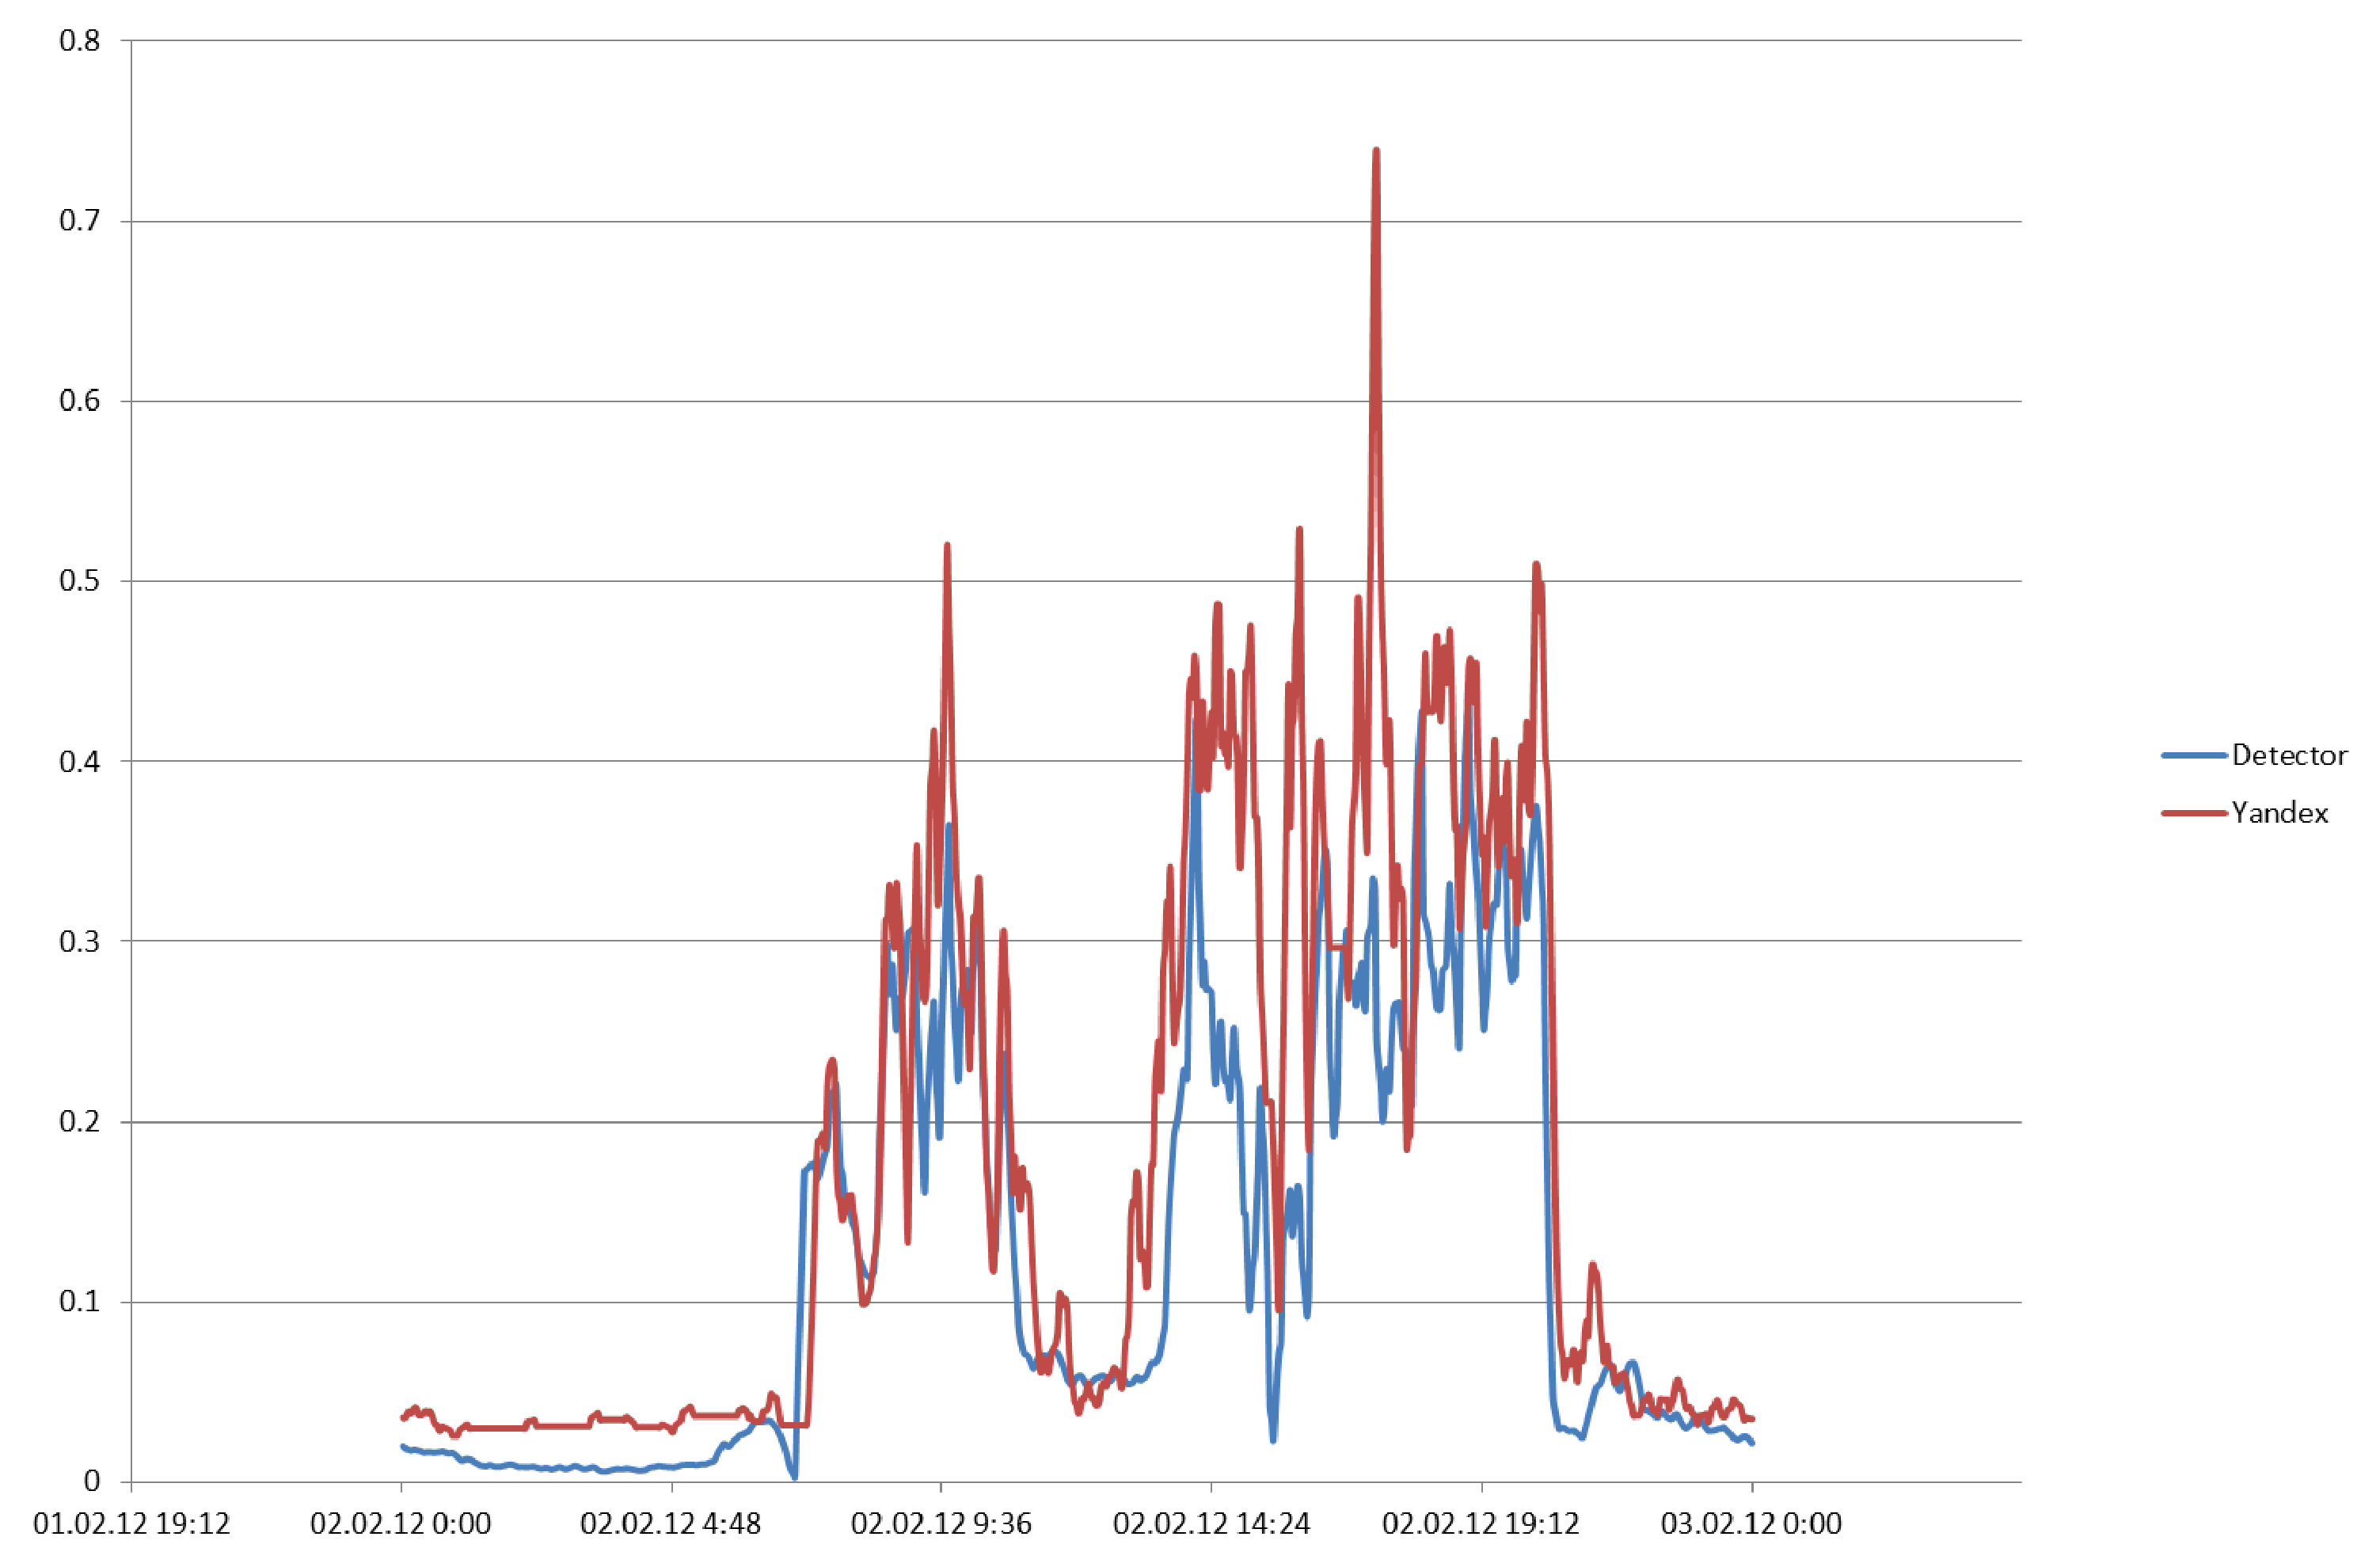
\includegraphics[width=0.9\linewidth]{Complex_Data_N.eps}
\caption{Плотность АТС для результатов обучения моделим~\eqref{eq::model_N}.}
\label{fig:cN}
\end{center}
\end{figure}
\begin{figure}[!ht]
\begin{center}
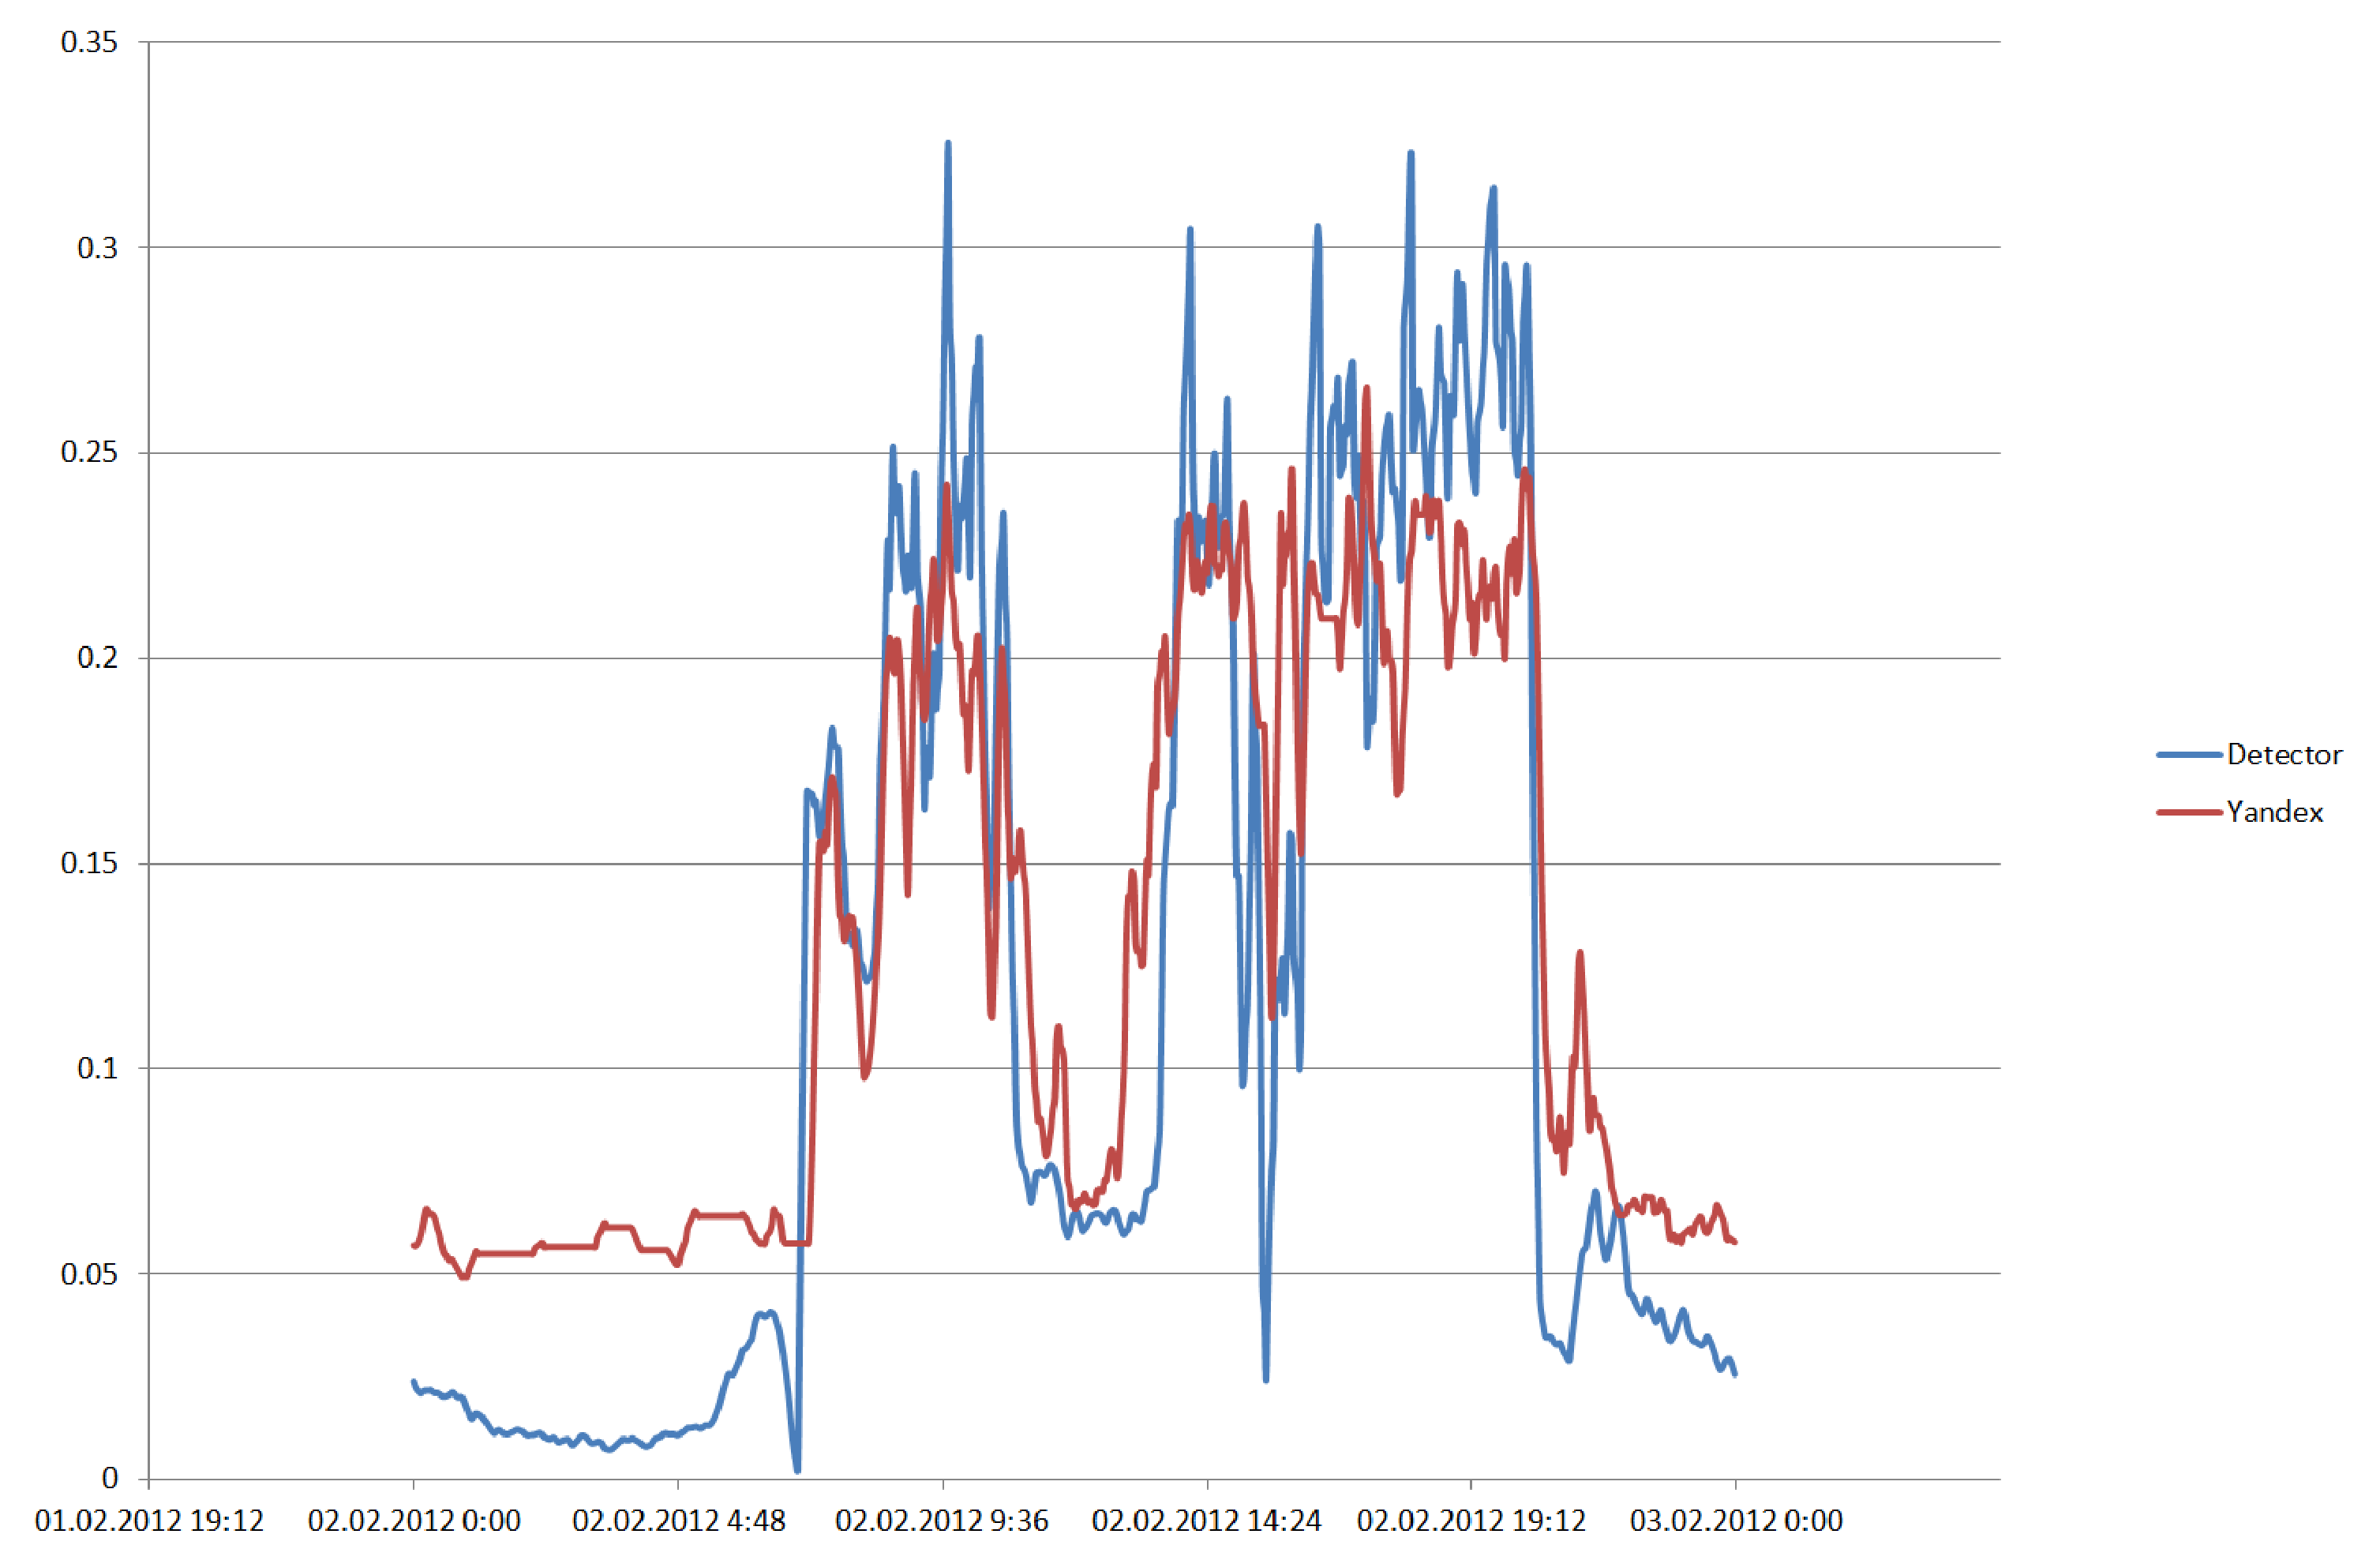
\includegraphics[width=0.9\linewidth]{Complex_Data_N_V.eps}
\caption{Плотность АТС для результатов обучения модели~\eqref{eq::model_NV}.}
\label{fig:cNV}
\end{center}
\end{figure}
\begin{figure}[!ht]
\begin{center}
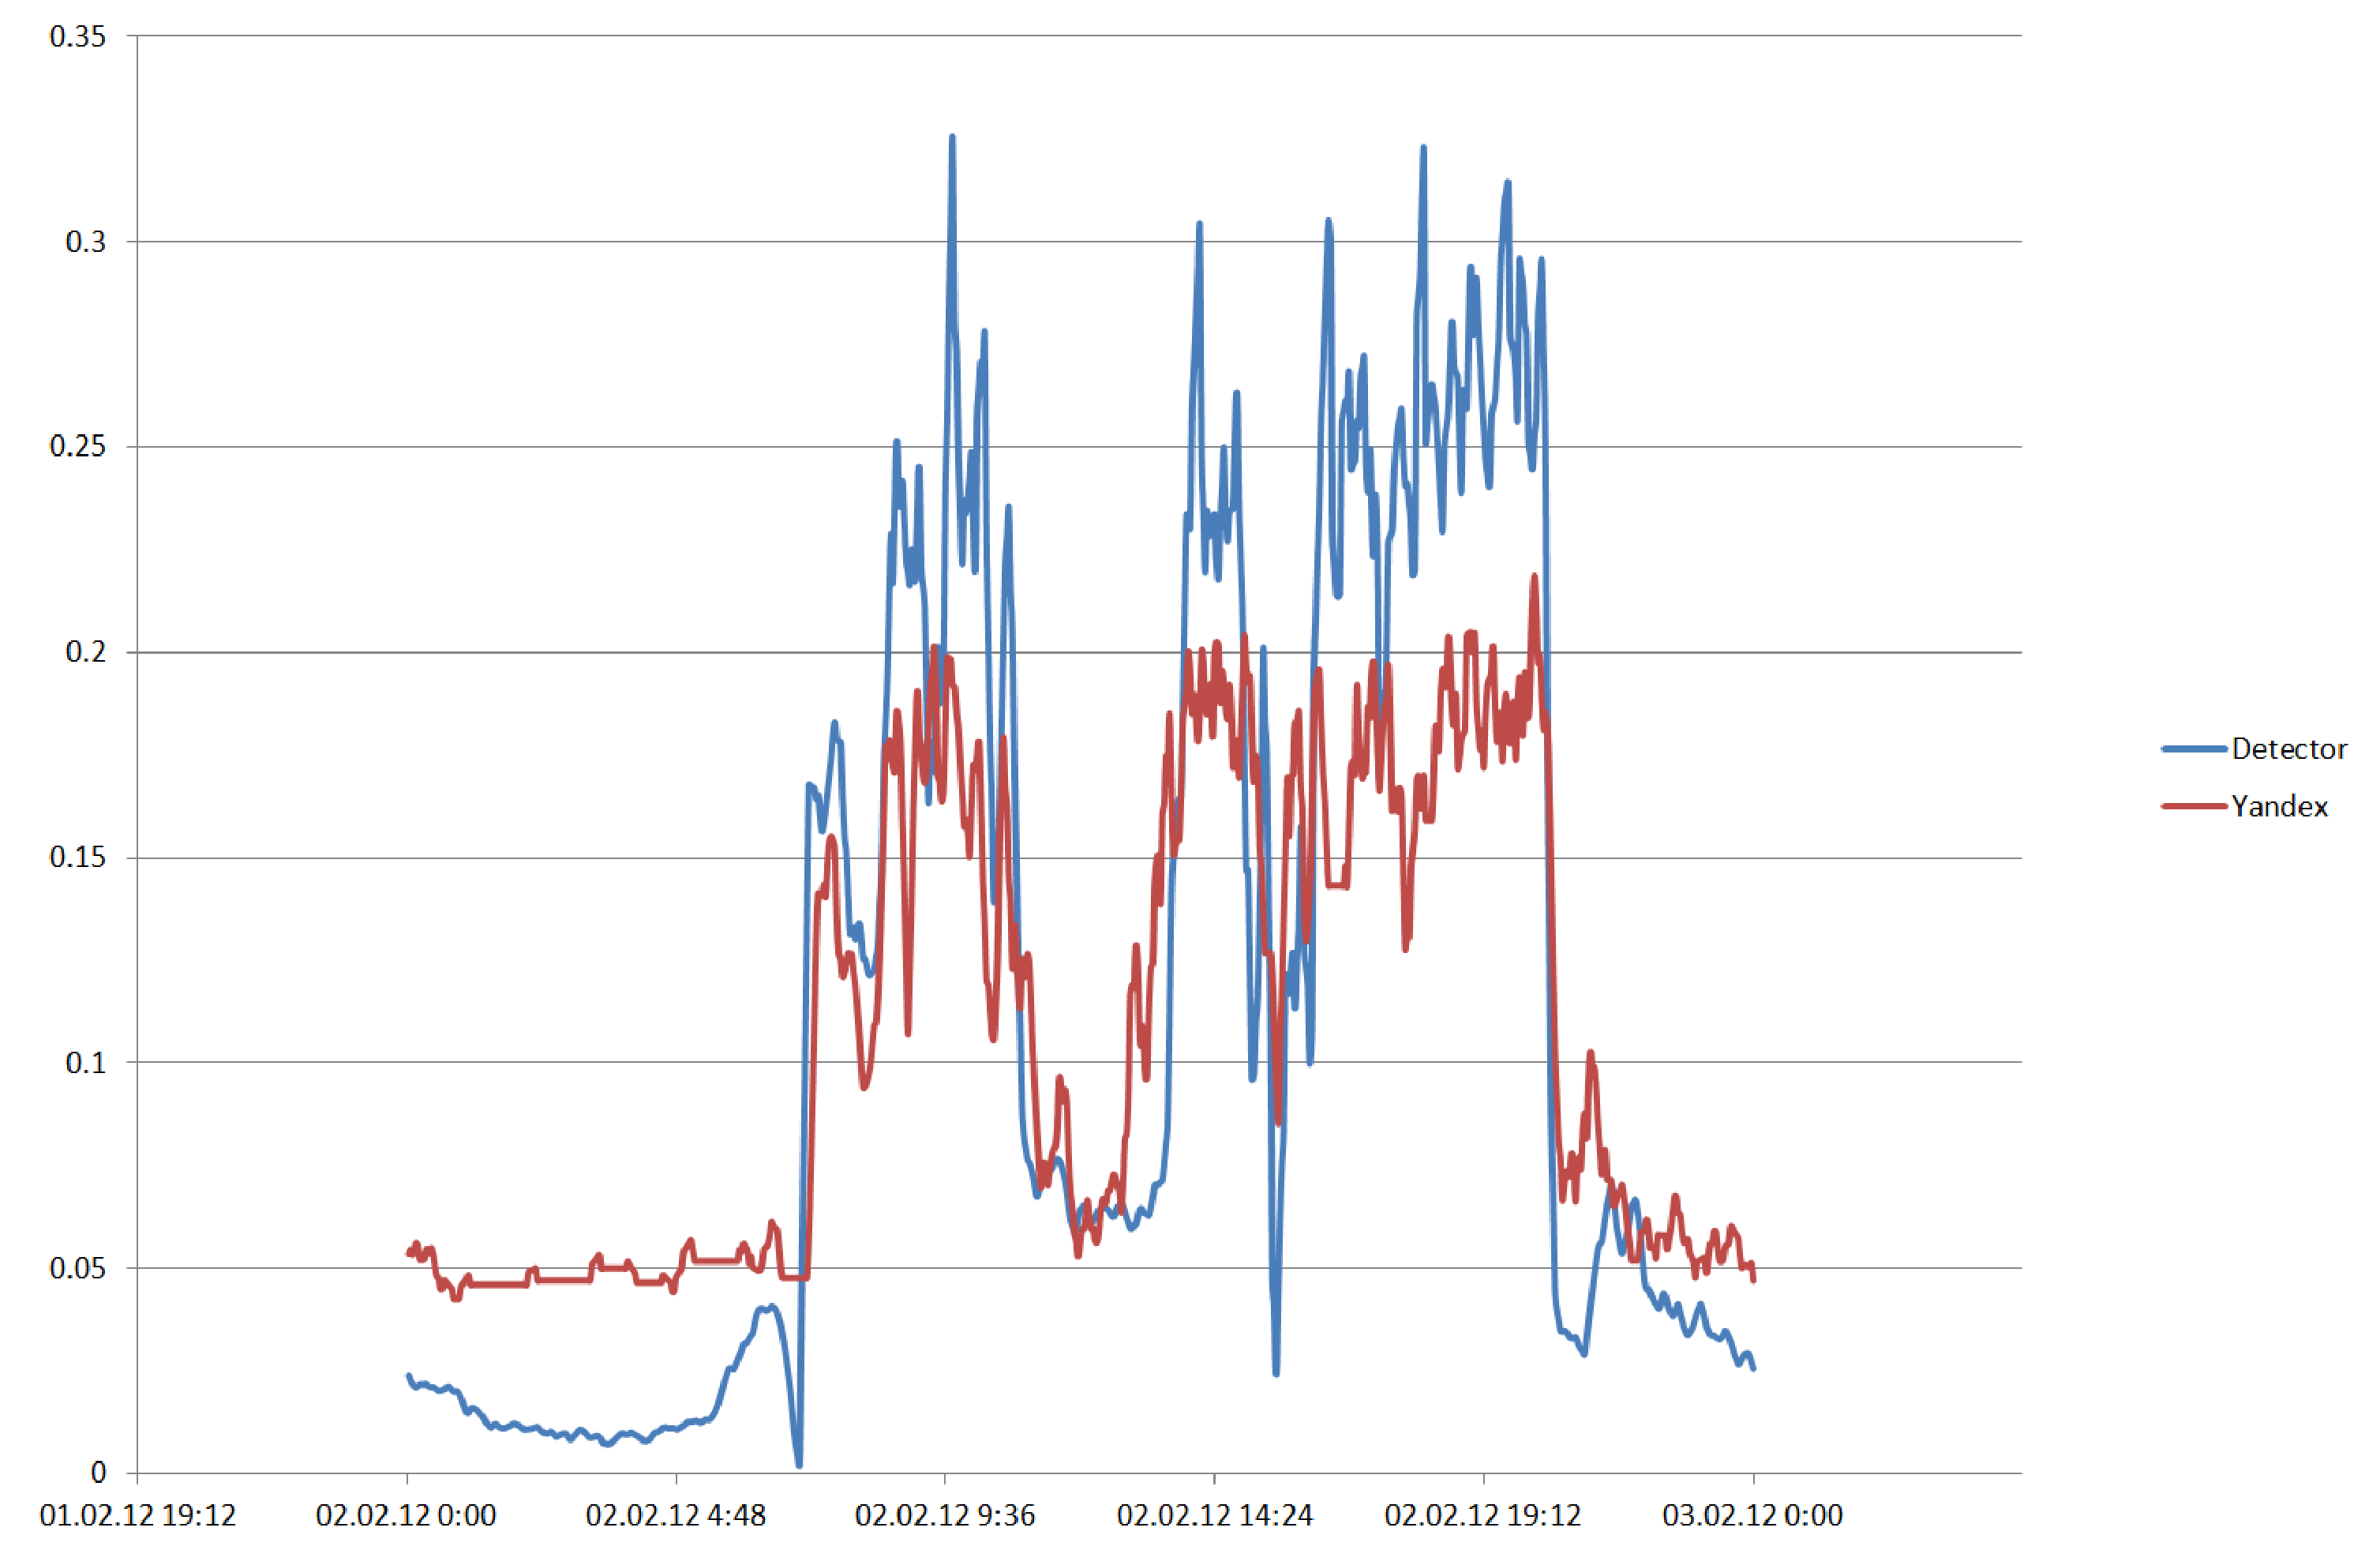
\includegraphics[width=0.9\linewidth]{Complex_Data_logN_V.eps}
\caption{Плотность АТС для результатов обучения модели~\eqref{eq::model_logNV}.}
\label{fig:clogNV}
\end{center}
\end{figure}
\begin{table}[!ht]
    \centering
    \caption{Сравнение моделей при всех значениях плотности $\rho_\text{det}$}
    \resizebox{0.85\columnwidth}{!}{
    \begin{tabular}{|c|c|c|c|c|}
         \hline
         & Модель~\eqref{eq::f_form} & Модель~\eqref{eq::model_N} & Модель~\eqref{eq::model_NV} &  Модель~\eqref{eq::model_logNV} \\
         \hline
         Среднеквадратическая ошибка & \textbf{0.03} & 0.031 & 0.0326 & 0.0314\\
         \hline
         Корреляция & \textbf{0.787} & 0.781 & 0.765 & 0.78 \\
         \hline
    \end{tabular}
    }
    \label{tab::model_compare}
\end{table}
\begin{table}[!ht]
    \centering
    \caption{Сравнение моделей при плотности $\rho_\text{det}>0.2$}
    \resizebox{0.85\columnwidth}{!}{
    \begin{tabular}{|c|c|c|c|c|}
         \hline
         & Модель~\eqref{eq::f_form} & Модель~\eqref{eq::model_N} & Модель~\eqref{eq::model_NV} &  Модель~\eqref{eq::model_logNV} \\
         \hline
         Среднеквадратическая ошибка & \textbf{0.058} & 0.119 & 0.065 & 0.093\\
         \hline
    \end{tabular}
    }
    \label{tab::model_compare_high}
\end{table}


\subsection{Эксперимент на въездах и съездах}
Приведем на примере двух перекрестков результат восстановления числа въехавших АТС за 02.02.2012 года.
На одном из перекрестков датчиками закрыты все въезды и выезды кроме одного въезда, результат работы алгоритма~\ref{alg::balance} представлен на рис.~\ref{fig:recex1}.
На рис.~\ref{fig:recex1} показано, что результат работы алгоритма~\ref{alg::balance} (красная кривая) проходит в области, соответствующей сумме данных с датчика и данных с GPS-треков (зелёные точки), то есть ограничение в задаче~\eqref{eq::in_out_quest} выполняется с достаточной точностью.
\begin{figure}[!ht]
\begin{center}
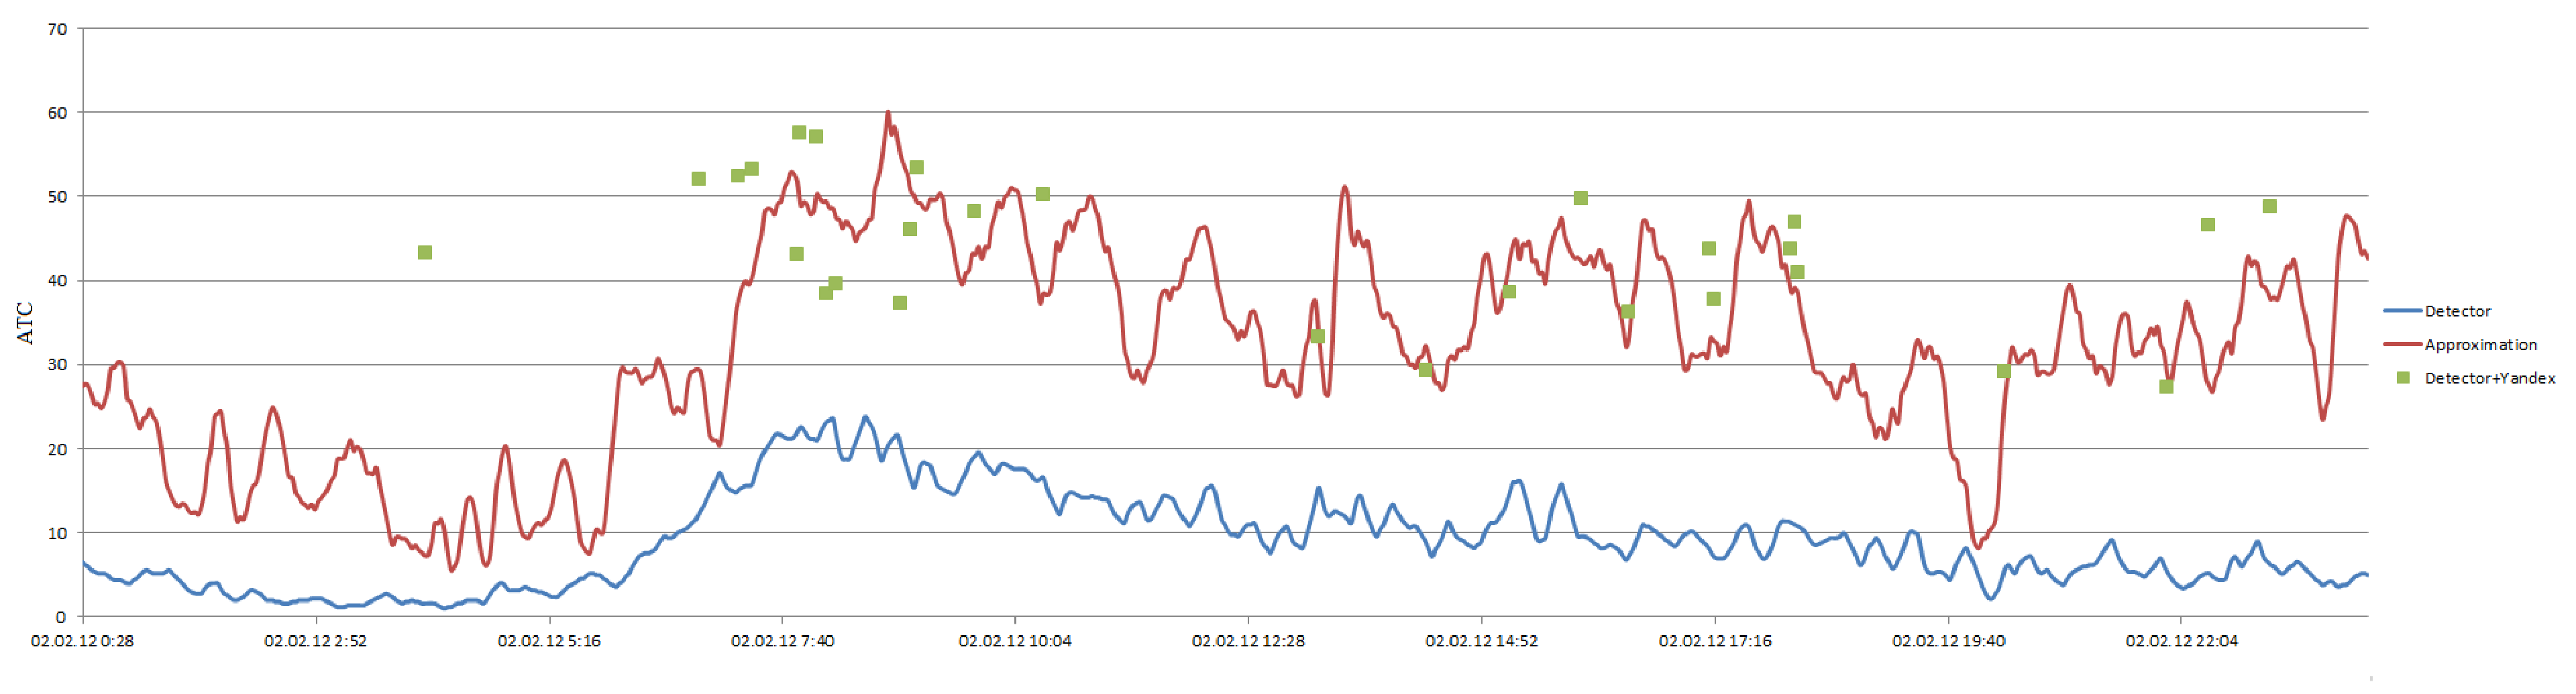
\includegraphics[width=1\linewidth]{recoveryexample1.eps}
\caption{Пример восстановления числа въехавших АТС. Синяя линия~--- число проехавших под датчиком на въезде АТС, зелёные точки~--- сумма данных с датчика и GPS-треков в моменты времени из множества $I_{in}$. Красная линия~--- восстановленные значения суммарного числа въехавших АТС $N_\text{estin}$.}
\label{fig:recex1}
\end{center}
\end{figure}

На втором перекресткe датчиками закрыты оба въезда, но один из датчиков фиксировал проехавшие АТС полчаса за день (до пяти АТС) и этот въезд был также включён в множество $K_\text{intrack}$, данных же трекого типа на данном въезде нет, результат работы алгоритма~\ref{alg::balance} представлен на рис.~\ref{fig:recex2}.
На рис.~\ref{fig:recex2} показано, что результат работы алгоритма~\ref{alg::balance} (красная кривая) проходит в области, соответствующей сумме данных с датчика и данных с GPS-треков (зелёные точки), то есть ограничение в задаче~\eqref{eq::in_out_quest} выполняется с достаточной точностью.
Также на рис.~\ref{fig:recex2} показано, что $N_\text{estin}$ в большинство двухминутных интервалов отличается от данных закрытого датчиком въезда (синяя кривая) менее чем на 5 АТС, а иногда полностью совпадает с ним.
Таким образом, данные с закрытого плохим датчиком въезда подтверждаются (малое число зафиксированных АТС), а также становится понятна причина отсутствия данных трекового типа на данном въезде~--- слишком слабый поток АТС.
\begin{figure}[!ht]
\begin{center}
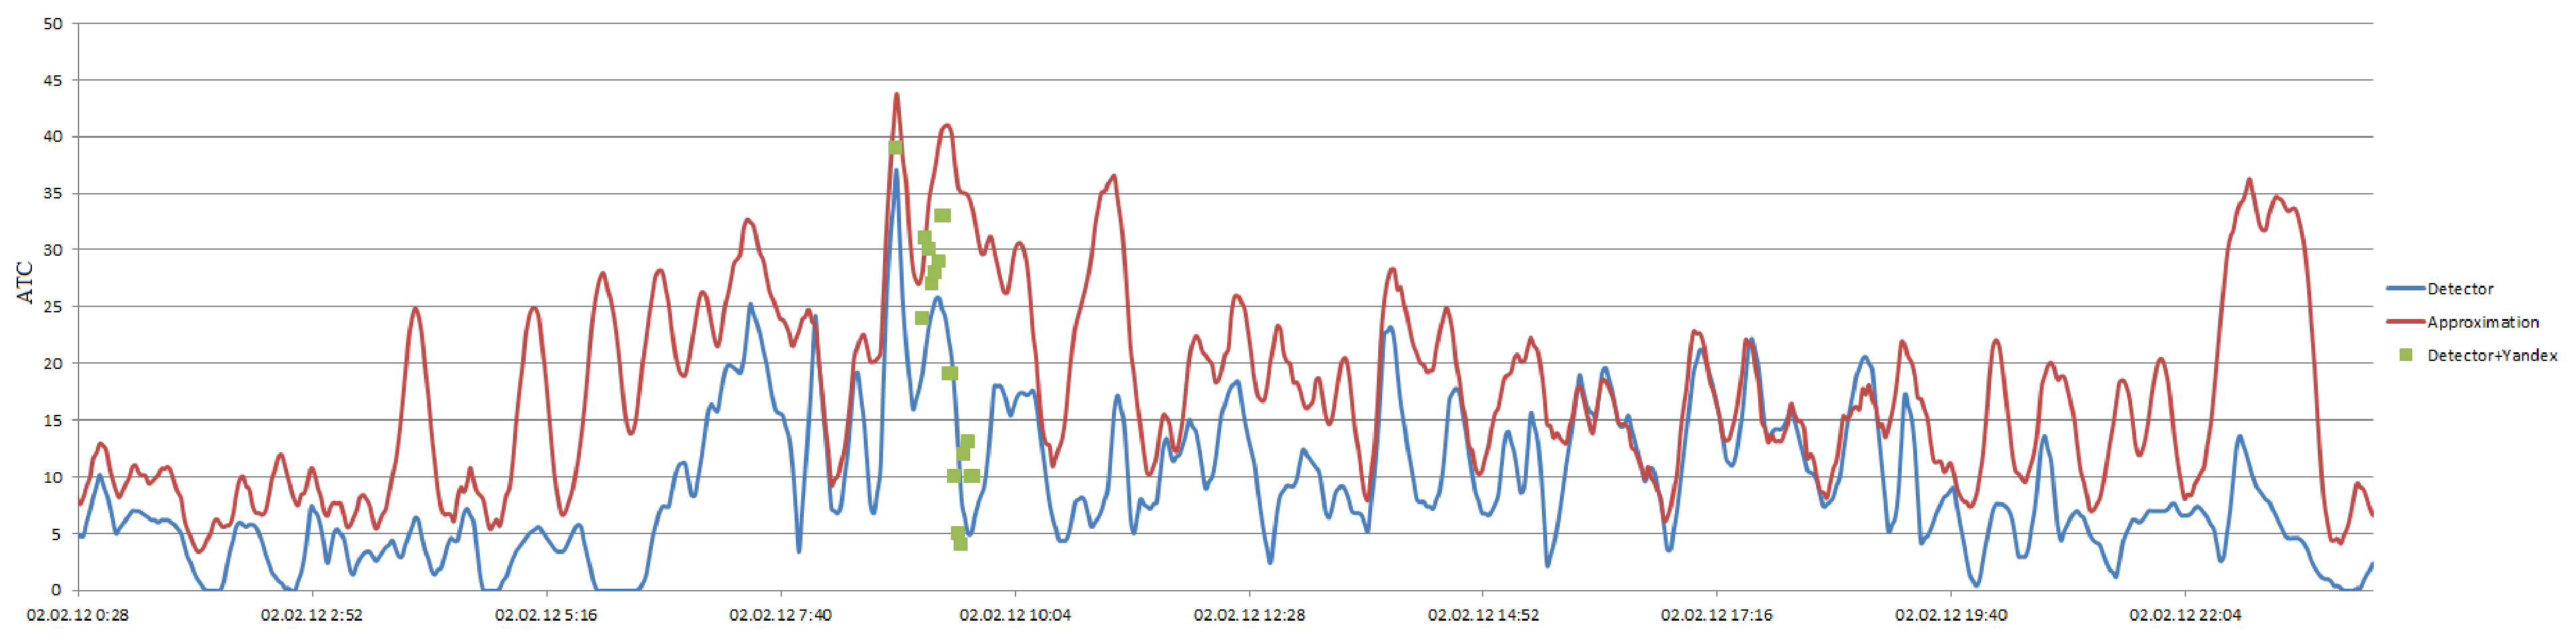
\includegraphics[width=1\linewidth]{recoveryexample2.eps}
\caption{Пример восстановления числа въехавших АТС. Синяя линия~--- число проехавших под датчиком на въезде АТС, зелёные точки~--- сумма данных с датчика и GPS-треков в моменты времени из множества $I_{in}$. Красная линия~--- восстановленные значения суммарного числа въехавших АТС $N_\text{estin}$.}
\label{fig:recex2}
\end{center}
\end{figure}
Все значения на рис.~\ref{fig:recex1},\ref{fig:recex2} усреднены за 10 минут.

\FloatBarrier
